\documentclass[12pt,a4paper]{article}
\usepackage{hyperref}
\usepackage{color}
\usepackage{amsmath, amsthm, amssymb, amsfonts, verbatim}
\usepackage{graphicx}
\usepackage[table,x11names]{xcolor}
\usepackage{geometry}
\usepackage{subcaption}
\usepackage[numbers]{natbib}
\usepackage{authblk}
\usepackage{ragged2e}

\title{
Can diffusion alone explain brain-wide distribution of CSF tracers within 24 hours?
}

\renewcommand{\comment}[1]{\textcolor{red}{#1}}

\newcommand{\kam}[1]{\textcolor{blue}{#1}}
\newcommand{\fixme}[1]{\textcolor{orange}{#1}}
\newcommand{\lars}[1]{\textcolor{magenta}{#1}}
\def\mm2s{mm$\sp{2}$/s}

\renewcommand\Affilfont{\raggedright\small}
%\renewcommand*{\Affilfont}{\normalsize\normalfont}

\author{Lars Magnus Valnes$\sp{a}$, Sebastian K. Mitusch$\sp{b}$, Geir Ringstad$\sp{c,d}$, \\ 
Per Kristian Eide$\sp{d,e}$, Simon W. Funke$\sp{b}$, Kent-Andre Mardal$\sp{a,b}$  
}

\affil{$\sp{a}$Department of Mathematics, University of Oslo, Norway\\
$\sp{b}$Center for Biomedical Computing, Simula Research Laboratory, Lysaker, Norway \\
$\sp{c}$Division of Radiology and Nuclear Medicine, Department of Radiology, Oslo \\ \hspace{2pt} University Hospital - Rikshospitalet, Oslo, Norway. \\
$\sp{d}$Institute of Clinical Medicine, Faculty of Medicine, University of Oslo, Oslo, Norway\\
$\sp{e}$Department of Neurosurgery, Oslo University Hospital – Rikshospitalet, Oslo, Norway


}

\begin{document}
\maketitle

\begin{abstract}
The proposed glymphatic system suggests a new mechanism for waste clearance from the brain, and has sparked new research on Alzheimer's disease where one of the defining features
is that metabolic waste accumulate within the brain. The glympahtic hypothesis is still controversial
and several biomechanical modeling attempts attempts on microlevel have dismissed the system or its assumptions. 	
On the macroscopic level, however, there are several findings that supports that transportation solute transportation cannot be explained
by diffusion alone, which is the current prevailing theoretical foundation of brain waste management. In particular, 
previous calculation by ourselves in simplified geometries suggested that diffusion alone cannot explain the tracer distributions
seen in these novel MRI investigations over hours and days. 
In order to include the complex geometry of the brain as well as the heterogenous CSF flow around the brain, we 
employed the methods of partial differential constrained optimization in order to  the identify apparent diffusion parameters 
that best would correspond to the MRI images. Apparent diffusion coefficients that do not match the values those seen in corresponding 
DTI images would then indicate that diffusion is not sufficient to explain the CSF tracer distribution and would as such be supportive of the glymphatic system. 
The apparent diffusion coefficients are somewhat larger than what is found in DTI (42\% in grey matter and XX\% in white matter).  


%The recently proposed glymphatic system propose a new mechanism for waste
%clearance from the brain and has opened for a new paradigm in        
%research on Alzheimer's disease where one of the defining features
%is that metabolic waste accumulate within the brain. The glymphatic system is still controversial and while
%experimental investigations in rodents as well as novel MRI investigations in humans
%provide evidence for the existence of this system, a proper theoretical
%foundation is currently missing from the bio-mechanical point of view. In particular,
%a crucial question in the current debate is how much the system accelerate
%waste clearance when compared to extra-cellular diffusion alone. In this paper,
%we will therefore evaluate to what extent partial differential constrained optimization methods
%can be used to identify modeling parameters for glymphatic transport when we    
%assume that the underlying equation can be represented by a diffusion equation
%representing extra-cellular diffusion and possibly dissipation caused by the glymphatic system.
\end{abstract}
\section{Introduction}
In 2012, ~\citet{iliff2012paravascular} provided evidence for a new brain-wide circulation system proposed to be crucial in the waste clearance of the brain. As most types
of dementias are associated with accumulation of metabolic waste within the brain, the new theory is potentially of fundamental importance for
the pressing challenges of dementia in the aging population. The circulation system is called the glymphatic system as it resembles the lymphatic system in the 
rest of our body and the 'g' highlight the importance of the glia cells. Evidence was given that the activity of the glymphatic system increases during  sleep by ~\citet{xie2013sleep}, thus linking sleep to clearance of toxic substances from the brain. 

The system proposes that 
the interplay between the cerebrospinal fluid (CSF) and the CSF-filled channels surrounding the vasculature of the brain, traditionally called Wirchow-Robin spaces, are crucial to  
facilitate clearance of waste.  
The glympahtic system is still controversial and several computational modeling studies have dismissed the system.  
For example, the previous studies~\cite{holter2017interstitial, smith2017glymphatic} suggest that diffusion dominates in the interstitium. Furthermore, ~\cite{asgari2016glymphatic, brynjfm, Diem} have found that dissipation in the paravascular spaces adds less than a factor two to diffusion for solute transportation. All these studies, however, concern the fluid transportation on the microlevel. 

On the macroscopic level, using imaging, it is however less clear that diffusion alone provides an adequate explanation. 
In \cite{iliff2013brain} a procedure for  investigate paravascular transport was proposed  and tested in a rat's brain. The procedure involved injecting a 
MRI-contrast into the CSF and subsequently image the transportation of the MRI-constrast at multiple time-points during a few hours after the injection.  
The procedure was extended to humans for the first time 
in 2015 by \citet{eide2015mri} where MRI images where acquired during 48 hours after the injection and quantified in a region-specific manner in 2018 \citet{ringstad2018brain} in individuals with dementia and controls. Overall, the MRI-contrast transportation  showed a centripetal and delayed pattern in individuals with dementia as compared with controls~\citet{ringstad2018brain} which showed a more centrifugal pattern. It was noted that the CSF-tracer transportation appeard faster than what can be expected from diffusion in simplified geometries. However, it was noted that the geometry of
the brain is quite complex and for instance the surface-to-volume ratio is fivefold that of a ball. 

The properties of the extracellular diffusion are well-known due to seminal work of Nicholson and colleagues, see~\cite{sykova2008diffusion} for an overview, and is fundamental to for  diffusion tensor imaging (DTI). 
It has been shown that diffusion coefficients in young and healthy subjects in white matter is around $0.7-0.9\times 10^{-3} \mathrm{mm\sp{2}/s}$ \citet{Helenius194},
while subjects with dementia typically have higher value and variation \cite{goujon2018can}. 
For larger molecules such as albumin (65-70 kDa) \citet{cserr1971physiology} estimated that transport by diffusion of a distance of 1 cm would require more than a hundred hours
and is therefore deemed to slow for the high demands of the brain.  
The crux of the glymphatic system is as such the fact that conventional DTI imaging is well explained by the traditional view of transportation by extracellular diffusion. 
However, the paravascular compartments are small, probably less than the vascular compartment that occupy around 3\% of the brain volume. As such, 
due to its small volume, the paravascular compartment may be dominated by the extracellular compartment at short time-scales, while still being a
significant contributor on longer time scales such as those in \cite{ringstad2018brain}. 

%In \cite{ringstad2018brain} brain-wide distribution of MRI-contrast was demonstrated during 24 hours after lumbar contrast injection. Brain-wide distribution by diffusion alone was deemed unlikely by the authors. The argument was based on analytical considerations where it was calculated that 50\g contrast enrichment would occur after 
%55 hours if planar diffusion can be assumed. However, 
%the surface of the brain is folded and is around five times larger than 
%a corresponding surface of a ball with the same volume. The increased
%surface-volume ratio of the brain increases the transportation efficiency.  
%On the other hand the contrast in the surrounding cerebral spinal fluid (CSF) is heterogeneous
%and changes significantly during the 24 hours of the investigations. 
%The heterogeneous distribution decreases the transportation efficiency as the amount of CSF tracer
%at times is very low. A third difficulty is that  
%MRI images were obtained only at a few time-points (around 10)  during the investigations in \cite{ringstad2018brain} which lasted 48 hours. 
%

On this background, our purpose in this paper is to assess the simple question whether the  
transportation seen in \cite{ringstad2018brain} can be explain by diffusion alone. In order
to include the complexity of the folding brain surface as well as the non-uniform CSF tracer distribution, we
will perform finite element simulations of the diffusion process combined with a parameter identification procedure. 
Thus we aim to investigate whether we can assess an effective diffusion coefficient on long time-scales (hours or days), by fitting a diffusion model to MRI data taken at multiple time-points in which the contrast is spreading through the brain. If the fit between observation and model is good and we identify diffusion coefficients that are 
in line with those predicted by DTI then paravascular transport can be ignored on the scale of our study. 
Our approach is to solve an optimization problem constrained by a partial differential equation (PDE) using the adjoint method where we have sparse observations on selected time-points, around 10 acquisitions during 24 hours, but through
the complete domain. 


There are really three questions that we want to answer.  
\begin{itemize}
\item Is the brain-wide distribution indicative of faster than diffusion transport? 
\item Is PDE constrained opt. a feasible approach (in terms of accuracy etc.)
\item Are the data of sufficient quality? 
\end{itemize}

%Hence, the challenges faced from a mathematical point of view 
%are that 1) the images are subject to noise, 2) resolution in space is limited to slightly less than 1 $\mathrm{mm}^3$ and 3)
%the sparse observations through the time domain. 
%Therefore we need to assess the sensitivity of the approach with respect to important factors, such noise levels and time resolution to determine whether this approach is a viable method to obtain parameters involved time-scales. 
%
%As such we need to assess the sensitivity of the approach with respect to important parameters such as the regularization parameters, noise levels and  time resolution to determine whether this approach is a viable method to obtain parameters involved time-scales. 
%We remark that the purpose
%of this paper is a systematic study of the mathematical challenges and that assessing  
%whether clearance is governed by a process that is faster than diffusion is not the topic of the current paper, 
%for that we would need to study several subjects. 

An outline of the paper is as follows. 
In Section 2 we present the methodology of the paper. Section 2.1-2.3 contains a detailed description of the medical imaging 
relevant to this study as we do not expect the reader to have prior knowledge of medical imaging. Section 2.4
describes the PDE constrained optimization problem and the corresponding solution algorithm, while 2.5 presents
a test problem using a manufactured solution that is used for method verification. Section 2.6 describes the implementation 
in FEniCS \cite{LoggMardalEtAl2012a}. In Section 3 we present the results and have a rather extensive discussion of the verification performed
using a manufactured solution (Section 3.1) before we present the results obtained by real observations in Section 3.2.1    
and a comparison with DTI data in Section 3.2.2. Finally, in Section 4, the methodology and results are discussed.  
   
\section{Methodology}

Sections 2.1-2.3 briefly describe the details of the imaging relevant for this study. More details on the MRI protocols can be
found in e.g. \cite{ringstad2018brain}. Sections 2.4-2.5 describe the solution of PDE constrained optimization problems and
its implementation in FEniCS. The exposition is, however, brief and we refer to e.g. \cite{hinze2008optimization} for more details. 



\subsection{MRI Data}
\begin{figure}
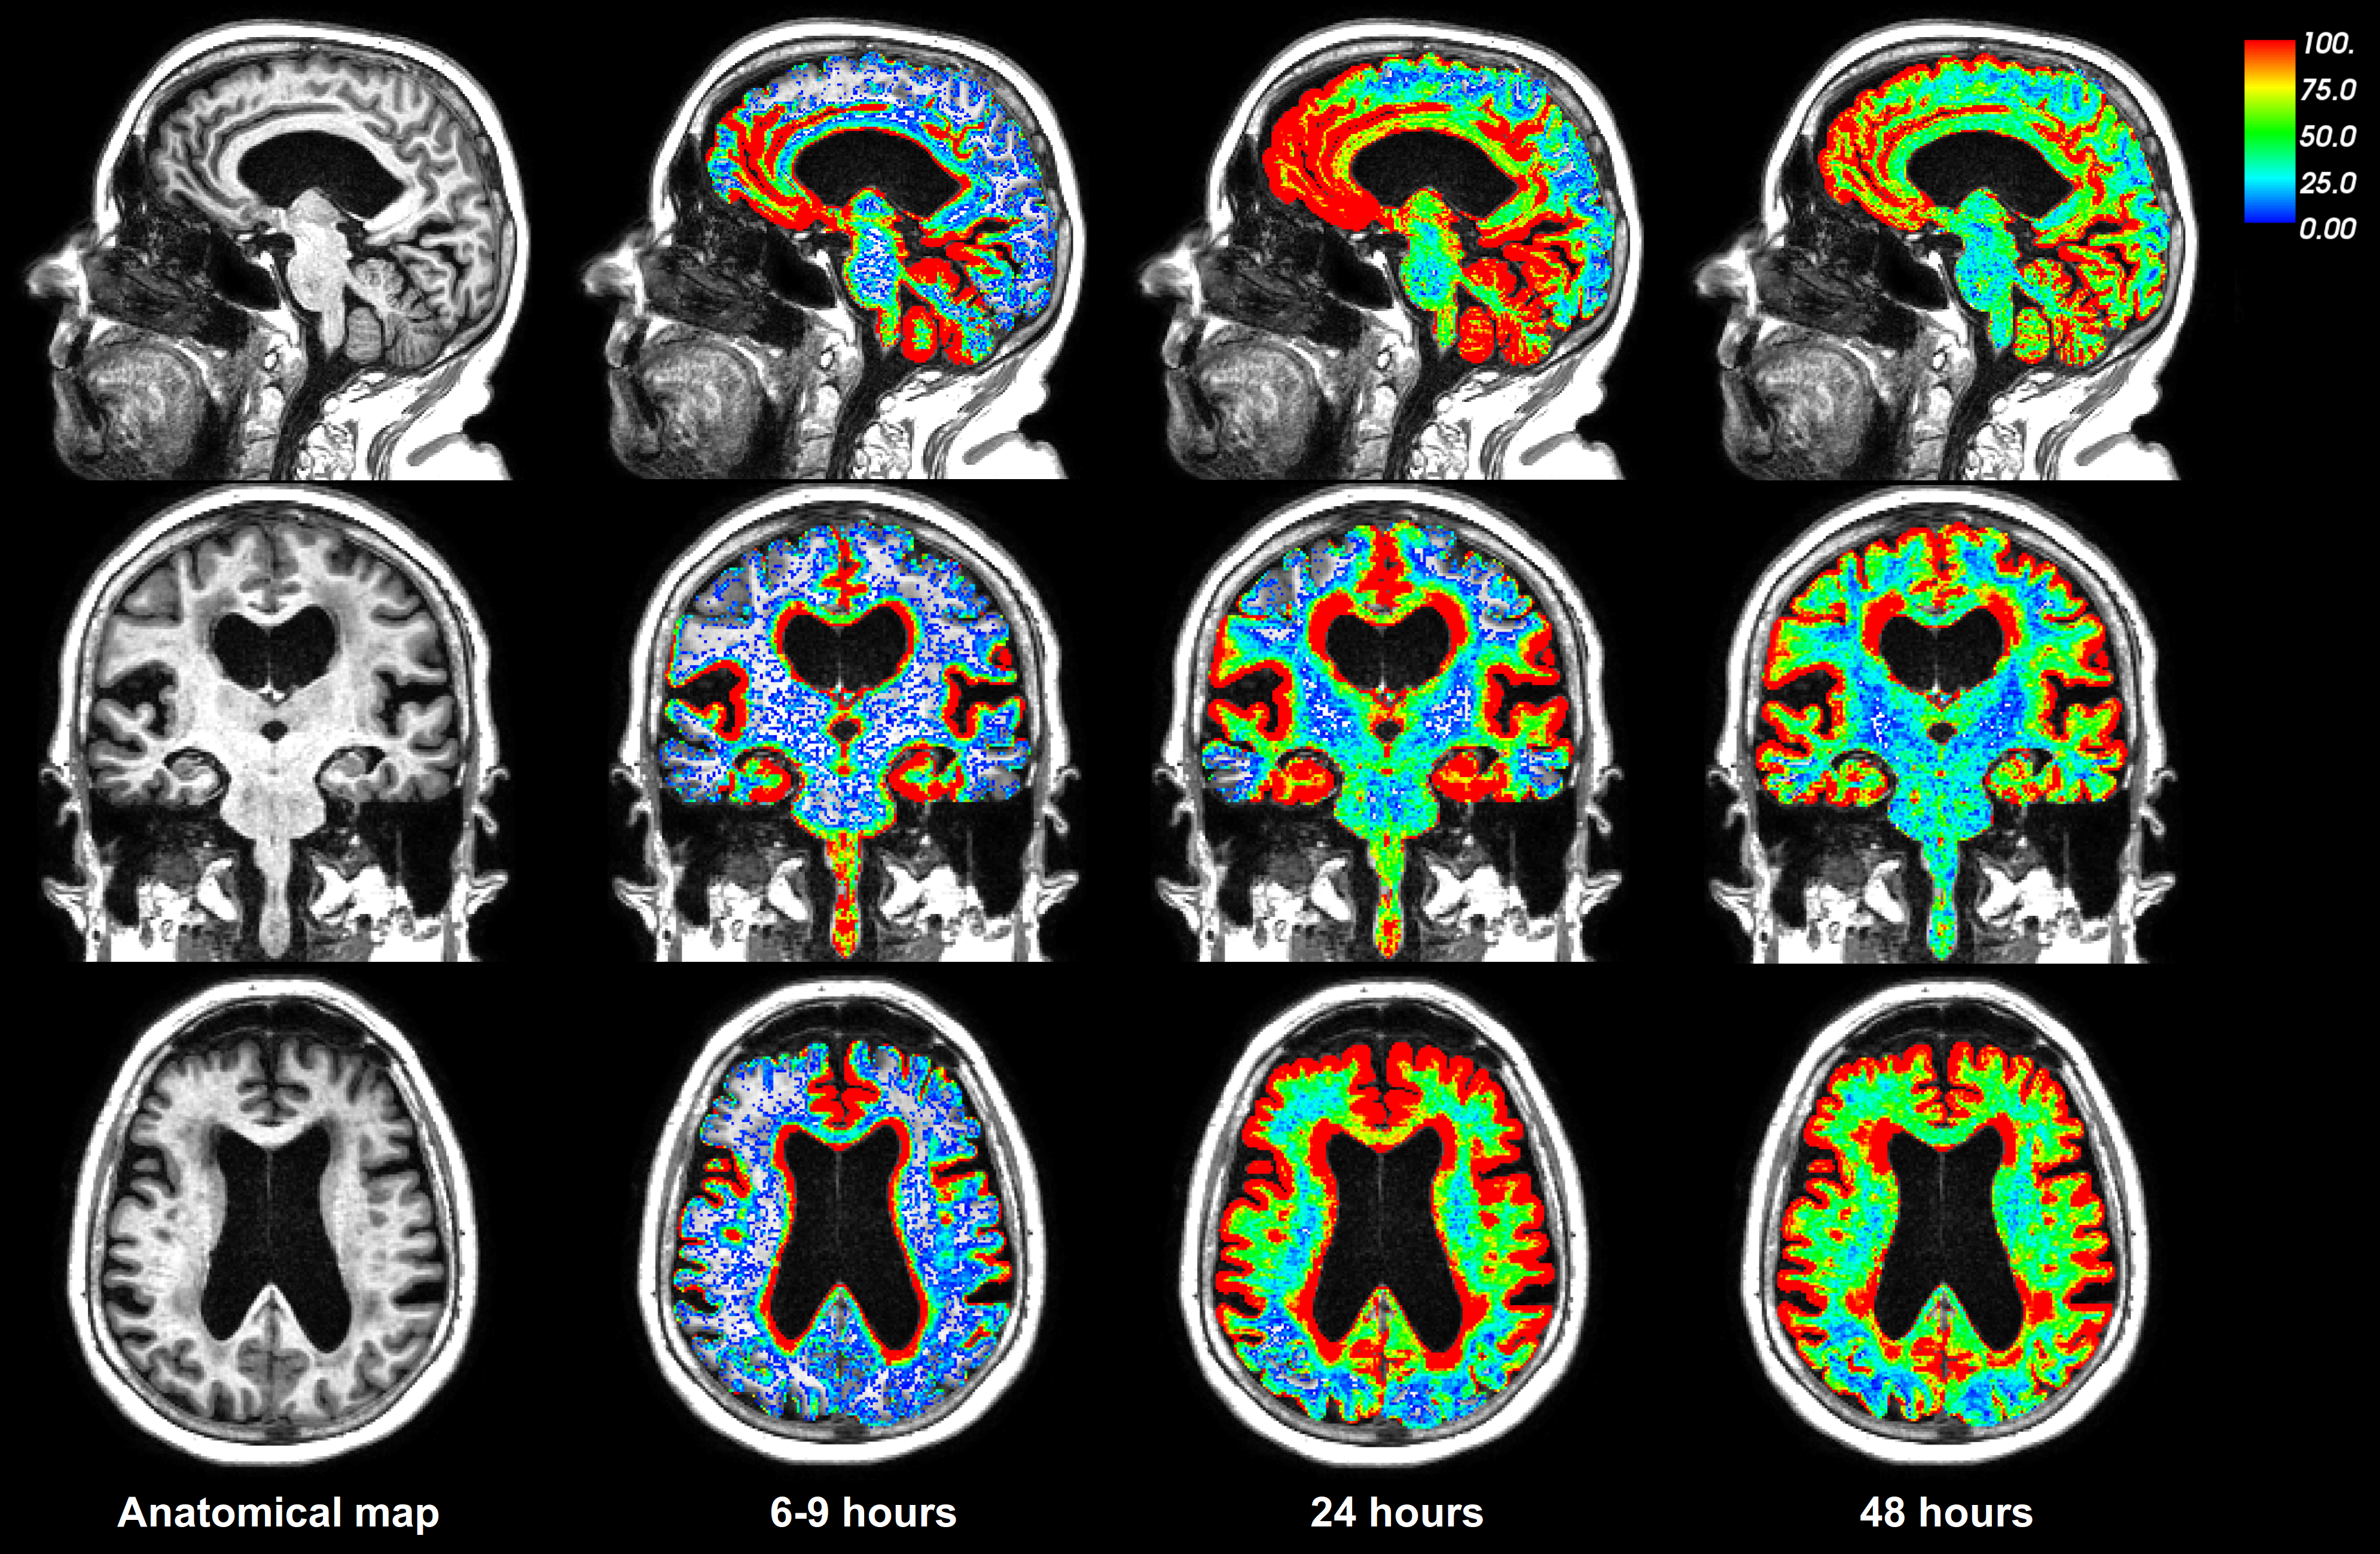
\includegraphics[width=0.95\textwidth]{../PatID-new-100.png} 
\caption{Shows the percentage change in T1 signal unit ratios from baseline at different observation times. The colorbar was restricted to the range $(0,100)$. }
\label{fig1} 
\end{figure}

\begin{figure}
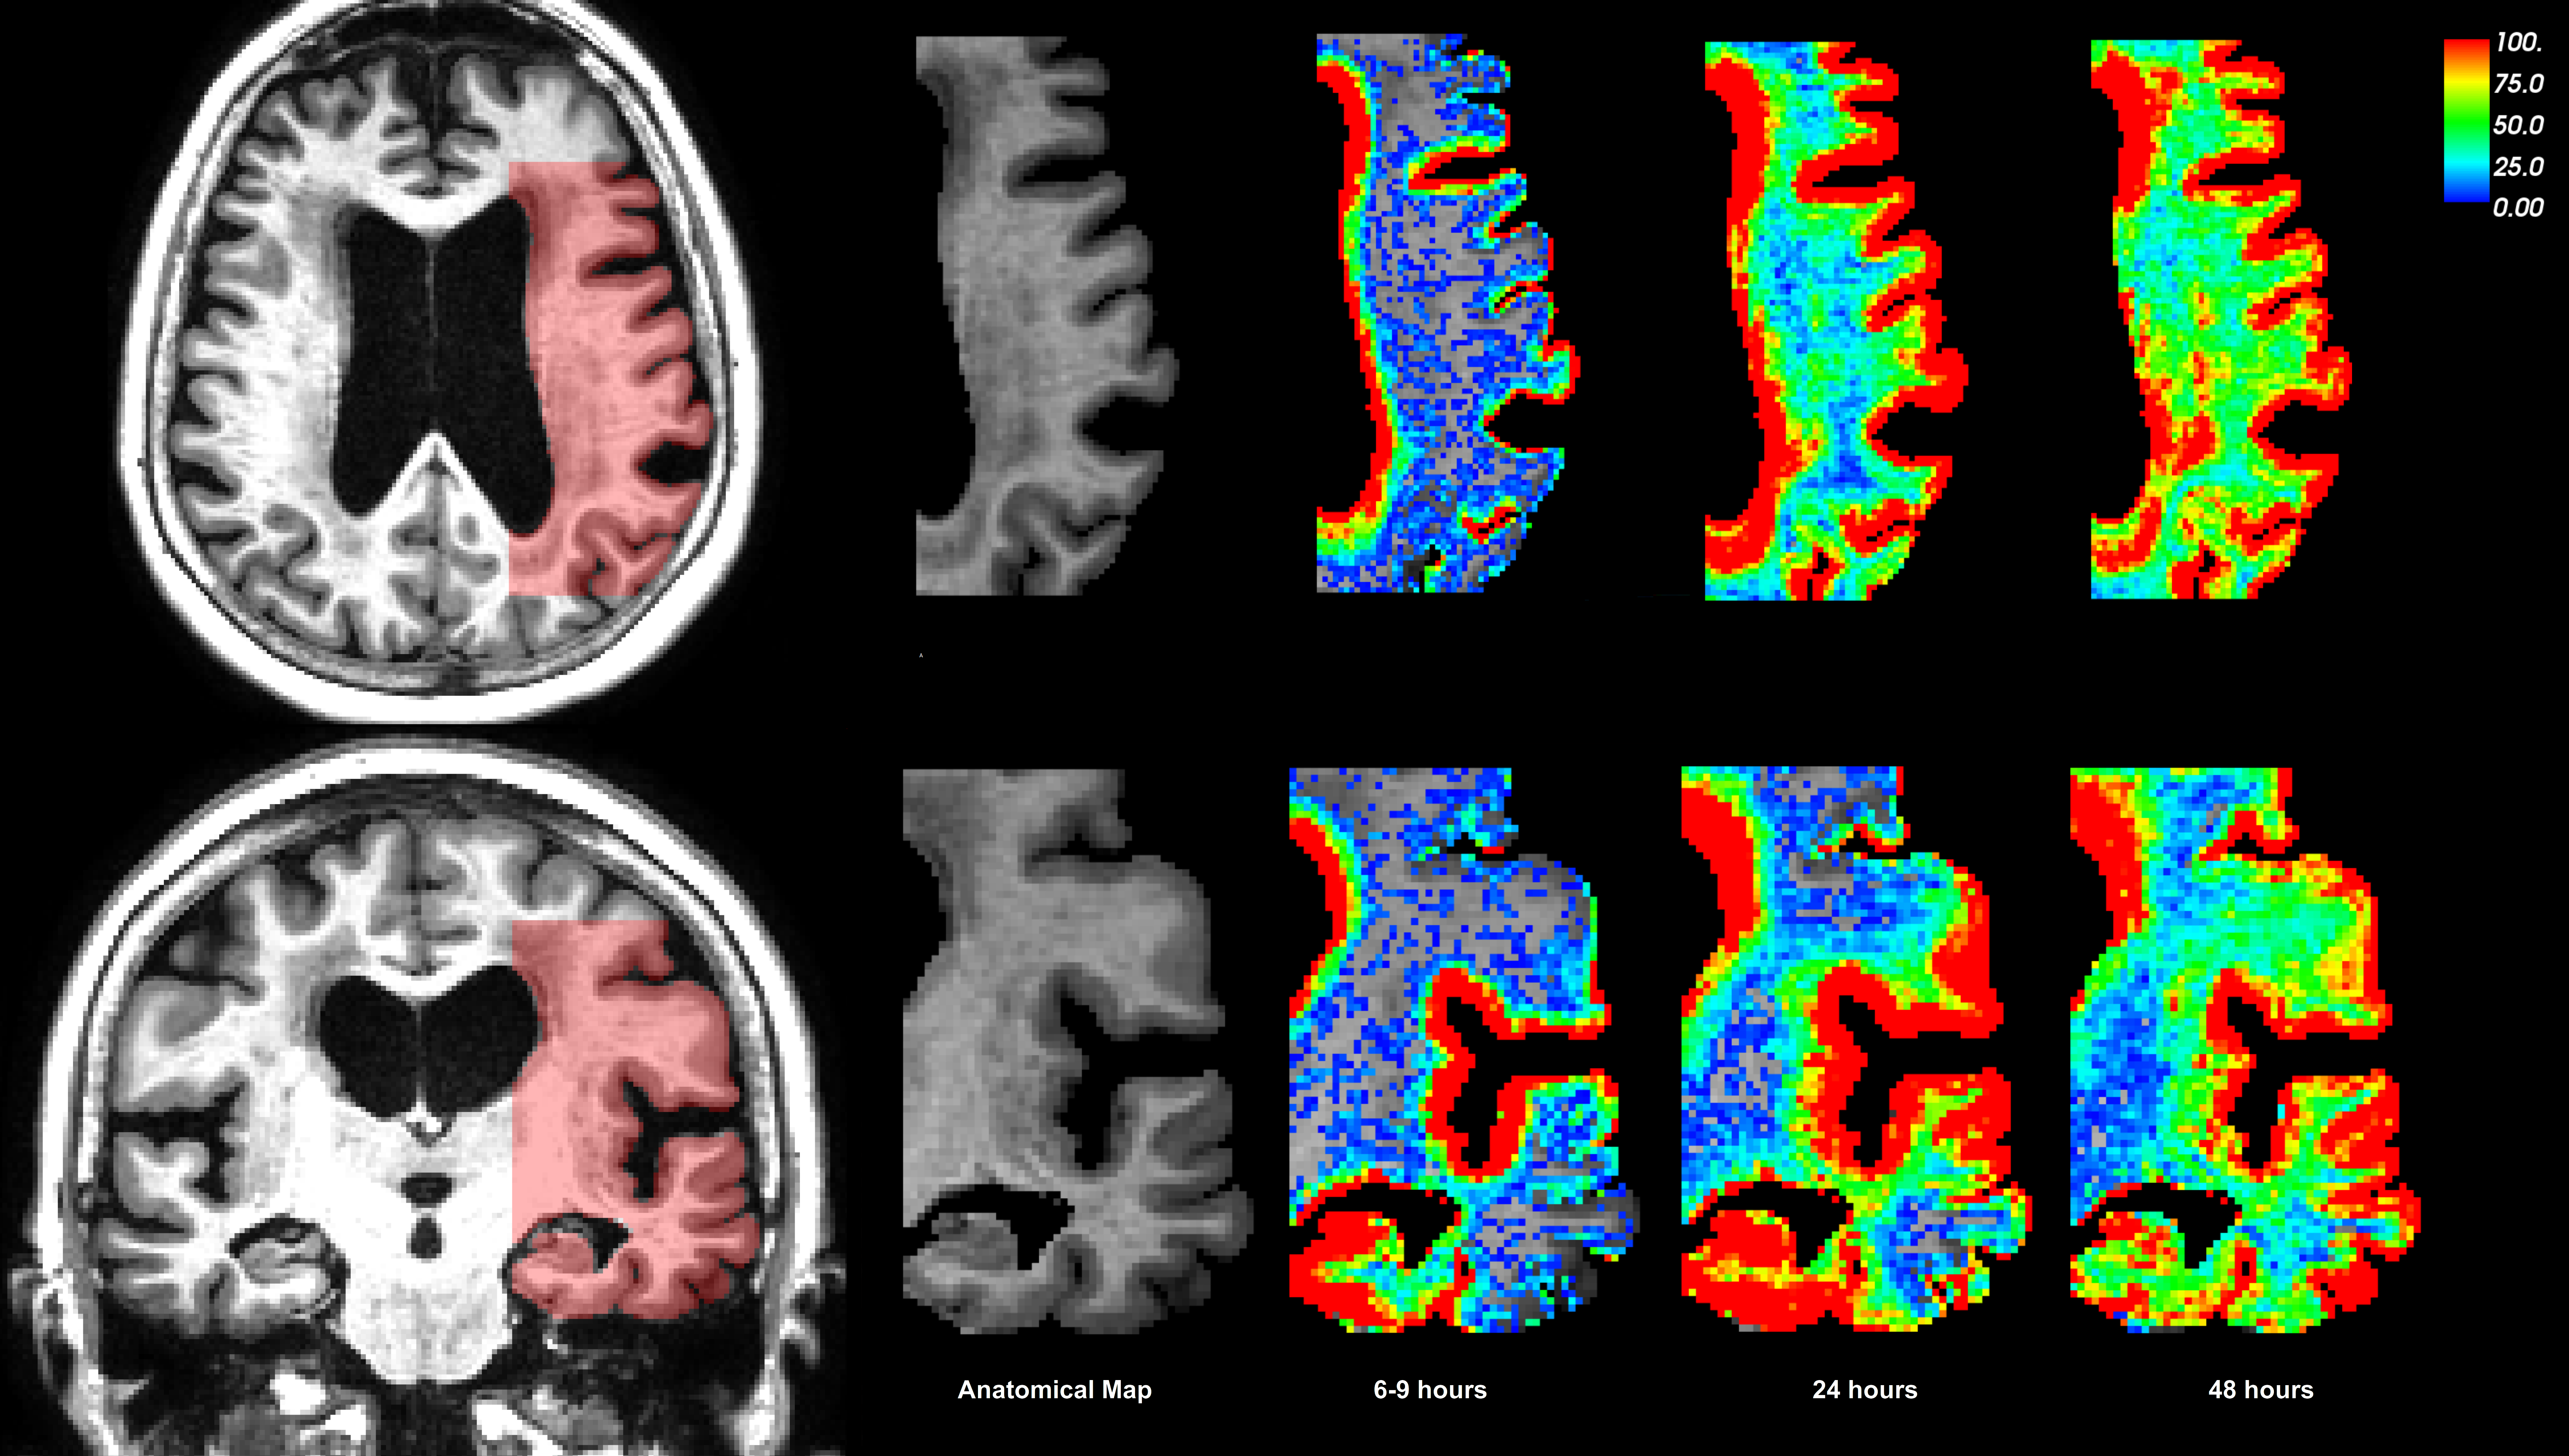
\includegraphics[width=0.95\textwidth]{../Zoom-PatID.png} 
\caption{Shows the percentage change in T1 signal unit ratios from baseline at different observation times in the slice (marked red in the left panel) used in the subsequent analysis. The color bar was restricted to the range $(0,100)$. }
\label{fig2} 
\end{figure}
Figure~\ref{fig1} shows distribution of MRI-contrast%CSF tracer
, as a percentage change in T1 signal unit ratios, see also~\cite{ringstad2018brain} for further information on the imaging procedure.   
Our data (not all shown) consist of a total of 10 MRI observations, including a baseline MRI taken before the contrast was injected. The observation points are distributed over 5 observations within 1-2 hours after injection, a single observation in the timeframes 2-4 hours, 6-9 hours, 24 hours and 48 hours. 
Figure~\ref{fig2} shows the region selected for our computations. 
The software Freesurfer \cite{Dale1999179, FischlLiuDale, spf2007, reuter:robreg10} was used to segment and align each of the observations, which made it possible to estimate voxelwise signal increase. 

%The MRI data was part of a larger study, which involves around 100 patients with the same MRI acquisitions. However, there are clinical differences in each patient, thus a thorough analysis is needed to obtain a robust and accurate method.


\subsection{Mathematical Model}
In \citet{sykova2008diffusion}, it was shown that the macroscopic diffusion in the brain can be considered a hindered diffusion with an apparent diffusion coefficient (ADC). The relation between the diffusion coefficients were defined as 
\begin{equation}
 \lambda =  \sqrt {D/D_{ADC}}
\label{tortuosity}
\end{equation}
with $\lambda$ denoted as the tortuosity.
In order to estimate the apparent diffusion coefficient involved in the contrast transportation shown in Figure~\ref{fig1} we assume that the process can be modeled by a diffusion equation. 
Then we constructed an optimization problem with the aim to minimize the difference between the observed and the modeled contrast distribution by optimizing the boundary conditions and the apparent diffusion coefficient. Thus enhanced transportation because of effects such as dissipation would result in an apparent diffusion coefficient larger than that predicted by DTI. The objective function was defined as 
\begin{equation}
\min_{D,g} \quad \sum\limits_{i=1}\sp{n} \int\limits_{\Omega} |u(t_i) - u_{obs}(t_i)|\sp{2} \mathrm{d}\Omega + \int\limits_{0}\sp{T} \int\limits_{\partial \Omega_1} \left( \frac{\alpha}{2} | g |\sp{2} + \frac{\beta}{2} \left| \frac{\partial g}{\partial t} \right|\sp{2} +  \frac{\gamma}{2}| \nabla g |\sp{2} \right) \mathrm{d}\Omega \mathrm{d}t  
\label{EQ::objf}
\end{equation}
subject to   
\begin{equation}
\begin{aligned}
\frac{\partial u}{\partial t} &=  \nabla\sp{2} u && \text{in} \qquad \Omega \times \left\lbrace 0 , T \right)  \\
u&=g && \text{on} \qquad \partial\Omega_1  \times \left\lbrace 0 , T \right) 
\end{aligned}
\label{Eq::PDE}
\end{equation}
Here, $u$ is the contrast distribution, $D$ is the apparent diffusion 
coefficient, $g$ is the boundary condition, $\Omega$ is the domain, and $T$ is the final simulation time. We assume that the domain $\Omega$ consists of three sub domains, each with a different diffusion coefficient. We denote the CSF (subarachnoid and lateral ventricle) domain as $\Omega_1=\Omega_{CSF}$, the grey matter as $\Omega_{GM}$ and the white matter as $\Omega_{WM}$. 
The apparent
diffusion constant is assumed to be constant within the CSF, grey and 
white matter but each region may have different values.  
The Dirichlet boundary condition is only applied on the outer facing boundary of the CSF domain, $\partial \Omega_1$. Homogeneous Neumann conditions are applied on the remaining boundaries.
The $\alpha$, $\beta$ and $\gamma$ parameters are non-negative regularization parameters 
and $u_{obs}$ are the observations at time-points $t_i$. 

The mesh construction was patient-specific and used the MRI of a patient diagnosed with idiopathic normal pressure hydrocephalus (iNPH). The software Freesurfer was used to segment and create the polyhedral surfaces of the white and cortical grey matter. Then the T2 weighted MRI \cite{ringstad2018brain} was used to segment the CSF compartment surrounding the cerebral and the lateral ventricles. CGAL \cite{cgal:rty-m3-18b} was used to combine the polyhedral surfaces and to construct the mesh. The computational requirement for the resulting mesh was significant, therefore two submeshes was also constructed, see Figure~\ref{Fig::Mesh}.
\begin{figure}
\centering
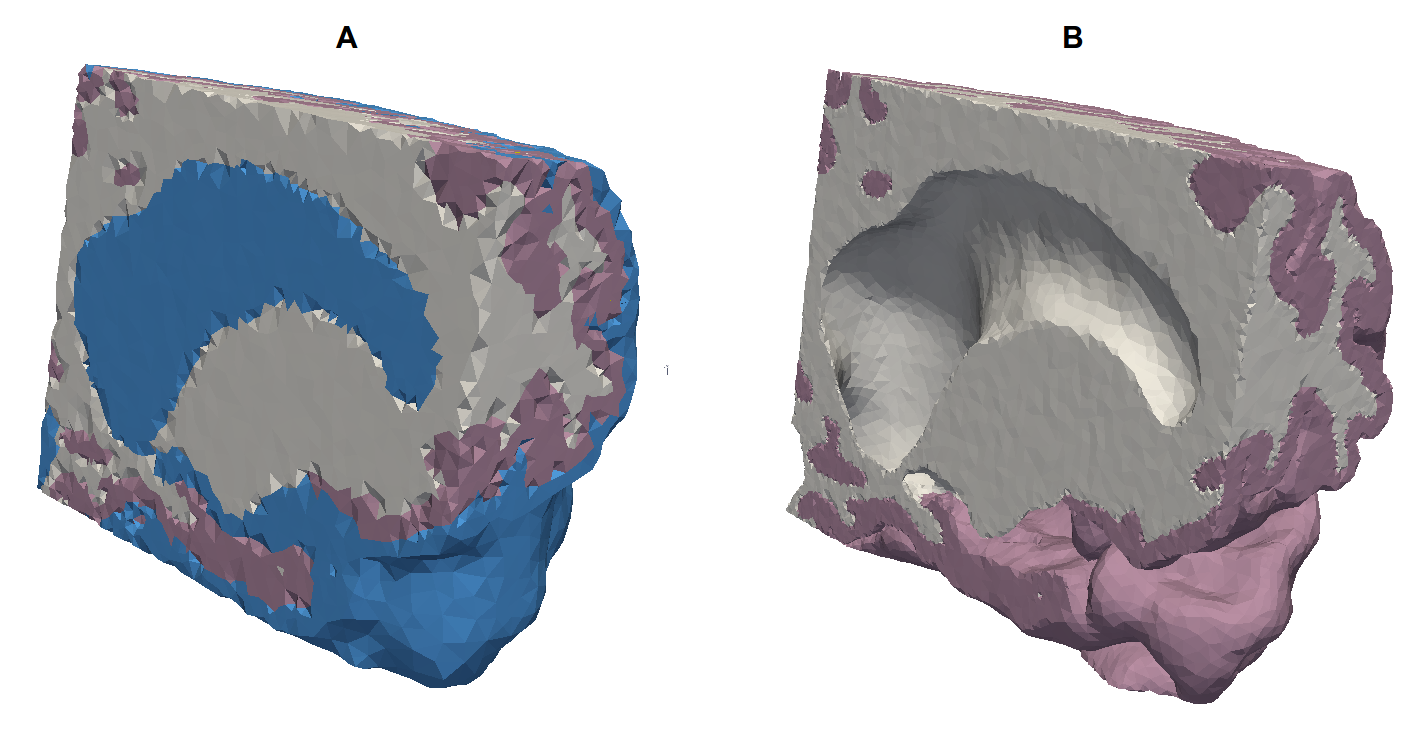
\includegraphics[scale=0.2]{../mesh.png} 
\caption{The leftmost image A) shows the mesh created from the baseline MR image with 3 domains, while the rightmost image  B) shows the mesh created from the baseline MR image with 2 domains. The blue domain corresponds to CSF domain, $\Omega_{CSF}$, the purple domain corresponds to grey matter,  $\Omega_{GM}$, and the white domain corresponds to white matter, $\Omega_{WM}$. }
\label{Fig::Mesh}
\end{figure}
The 3 domain mesh in Figure~\ref{Fig::Mesh} A, consists of 244318 tetrahedral cells and 22057 vertices, while the 2 domain mesh (without the CSF compartment) Figure~\ref{Fig::Mesh} B consists of 335589 tetrahedral cells and 73002 vertices. 

%\section{Numerical Experiments}
The process of estimating the diffusion coefficients in terms of the PDE constrained optimization problem \eqref{Eq::PDE} is complicated as appropriate parameters, i.e. $\alpha$, $\beta$ and $\gamma$,  have 
to be determined and robustness with respect to resolution and noise have to be assessed. Our approach was as follows. 

\textbf{Manufactored solution.}
In order to verify our code and assess the range of parameters suitable for simulation we performed a series of 
simulations with regularization parameters, discretization parameters and noise levels against a known manufactured solution. A total of 141 numerical experiments
where conducted. The details of the numerical tests can be found in the Supplementary \ref{sup:manu}. 

\textbf{MRI data.}
It can be seen from Figure ~\ref{SAS} that the boundary condition contains high frequent noise. This may be attributed to noise and small errors in sampling the MRI-data onto the mesh. The sampling error can be caused by miss-alignment between different observations, and by inaccuracy of sampling discontinuous voxel data. In more detail, the boundary surface is constructed by smoothing voxels to avoid sharp edges, this can cause the boundary vertices to correspond to voxels outside the select range of data. Therefore, we investigated three approaches to minimize the sampling error : 
\begin{itemize}
\item gradient regularization 
\item projection onto the boundary surface
\item Gaussian smoothing 
\end{itemize} 
 
The implementation of the gradient regularization required that the boundary was decomposed to avoid the boundary values being continuous over different subdomains. We decomposed the boundary as seen in Figure~\ref{markedboundaryvalues}, with the red and blue boundary adjacent to the CSF. We defined the red boundary $\partial \Omega_r$ and the blue boundary $\partial \Omega_b$ as Dirichlet boundaries, while the green and yellow were Neumann boundaries. The regularization parameter $\gamma$ was subsequentally to non-zero in Eq.~\ref{\label{EQ::objf}}. We initially tested gradient regularization with the same parameter $\gamma$ on both boundaries, but the different distribution of tracers on the boundaries made it difficult to find an adequate value. It was observed that the concentration in the lateral ventricles were more uniform than that in the SAS, so we defined $\gamma$ as
\begin{equation}
\gamma = \begin{cases}
0.01\tilde{\gamma}  \in &\partial \Omega_{b} \\ 
\tilde{\gamma} \qquad \in  &\partial \Omega_{r}
\end{cases}  
\end{equation} 
with $\tilde{\gamma}$ as the referenced, i.e. mentioned in the text, regularization parameter.

The projection method worked by selecting each boundary vertex on $\Omega_b$ and $\Omega_r$, then finding the corresponding voxel using an affine transformation. Then for each voxels, we  computed the average of all CSF segmented voxels in a two voxel vicinity. The averages was then set to be the observational value for corresponding boundary vertex in the computations.

We used the Gaussian smoothing found in the python-module scipy~\cite{jones2001scipy}, and applied the smoothing to the voxel based MRI-data. The smoothing function required that standard deviation of a Gaussian distribution was specified, which was tested in the range 0.3-1.5.


 %The projection and smoothing approach changes the observations, while the gradient regularization adds additional term to the functional. Therefore a dual method can also be considered, 
%It can be seen from Fig XX that the boundary conditions is noise. This may be attributed to noise or small errors
%in the segmentation/registration process where voxels close to the boundaries between the brain and CSF are miss-aligned
%by the sub-voxel segementation procedure. In particular, the surfaces can cut a voxel at any plane, not only the planes
%through the voxel vertices. We chose three approaches to handle this problem. \kam{Lars: kan du utbrodere litt her? 
%Jeg synes vi skal beholde også Fig 10 fra tidligere.  }   




\section{Results}

\subsection{Estimation of diffusion coefficients with a manufactured solution.} 
We first ran a series of tests of different $\alpha$ and $\beta$ for the manufactured solutions where we assumed observations every 2.4 hours
over the course of 24 hours. It was found that for $\alpha \in (10^{-6}, 10^{-2})$ and $\beta\in(10^{-6}, 10^2)$, the error in 
the diffusion coefficients of both CSF, grey and white matter was less than 7\%. Furthermore,  
$\alpha \in (10^{-6}, 10^{-2})$ and $\beta\in(10^{-6}, 10^{-2})$ gave errors of less than 1\%. Second, the robustness with respect noise
was investigated. The noise-amplitude was set to 0.3 which equals the initial condition of the manufactured solution
and 23\% of the manufactured solution at its max. The method was found robust with respect to the noise, as illustrated in the Supplementary Fig~\ref{12hourswithnoise}.  In fact, for  $\alpha \in (10^{-6}, 10^{-2}$ and $\beta\in(10^{-6}, 10^{-2})$ the error in the diffusion coefficients in CSF was less than 23\% and less than 9.7\% in grey and white matter. Because of the much larger 
error in the CSF compartment, we decided to re-mesh with a focus on the grey and white.
 
The convergence was monitored and shown in Figure~\ref{convergence}, and we can see the different regularization parameters have similar convergence for the diffusion coefficients. 
We had limited number of MRI observations available, so we also performed tests with variation in the number of time-steps and observations, which are documented in the Supplementary. These test used the same setup and parameters as the initial tests, and we analyzed the variation of number of time-steps and observations separately.
We selected the number of time-steps to 10 and 40, and the number of observations to be 5 and 20. We can see that in  Figure~\ref{boundarycontrol} an increase in the number of time-steps causes oscillations for $\alpha\gg\beta$. The test of 5 observations gave similar oscillation, which suggests that high ratios between time-steps and observations contributes to oscillations. This can be counteracted by selecting high values temporal regularization $\beta$ to enforce a smooth curve.  







% For instance, as seen by the the pink line for $\alpha=1.0$ and $\beta=0.0001$ the peaks corresponds to a observation.
%These oscillations occurs due to the spacial regularization $\alpha$, which minimize the value of $g$ between observation times. 




%\subsection{Estimation of diffusion coefficients with a manufactured solution.} 



\kam{Lars: skriv om resten av eksperimentene. Fig 6 og 7 bor med i Suppl}   

\subsection{Estimation of the diffusion coefficients from the MRI data} 

\subsubsection{Results obtained when using real observations}
The MRI data consisted of the observations at times $t_i$ distributed in the 48 hours time frame with the time $t_i=0.00$ \lars{zero?} as the first observation 1-2 hours after the contrast was injected. There was no significant visible change in the contrast between the observations the first 2 hours, therefore we used observation times listed in Table ??.

The estimation of contrast concentration proved difficult in the CSF compartment. Therefore the 2 domain mesh, shown in Figure~\ref{Fig::Mesh} was used in the computation. 

The boundary control was set to the external boundary of both domains, and the subscript in $D_{\Omega_{GM}}$ and $D_{\Omega_{WM}}$ denotes grey and white matter diffusion coefficients. Furthermore, bounds were added to the L-BFGS-B algorithm to ensure non-negative boundary controls and the convergence criteria was adjusted so that the optimization was stopped when the $L^\infty$-norm of the projected gradient of the objective functional dropped below $6.0\times 10^{-1}$. The other specific  computational parameters are listed in Table ??.
The results are shown in Table~\ref{Tab::Real-data}, and the observations after 12 and 48 hours were compared with the corresponding states in Figure~\ref{Fig::realdata}. From Table~\ref{Tab::Real-data}, it can be observed that $D_{\Omega_{WM}}$ has 24\% higher value on average for $\alpha =1.0\times 10^{-2}$. It can also be observed that the $D_{\Omega_{GM}}$ have a consistent increases with a decreasing $\beta$.

\subsubsection{Comparison with data obtained from DTI analysis}
The median diffusion coefficient in the DTI was estimated to be 
$8.7\times 10\sp{-4} \mathrm{mm\sp{2}/s}$ 
in white matter and 
$1.0\times 10\sp{-3} \mathrm{mm\sp{2}/s}$ 
in grey matter. This corresponds to a tortuosity of $1.85$ and $1.73$ given that the self-diffusivity of water has been reported/estimated to be around $3.0\times 10\sp{-3}\mathrm{mm\sp{2}/s}$ at $37\sp{o}C$. We estimated the diffusion coefficient of $3.8\times 10\sp{-4} \mathrm{mm\sp{2}/s}$ for Gd-DPTA, which gives an estimate for the apparent diffusion coefficient in the grey and white matter to be $ 1.3\times 10\sp{-4}\mathrm{mm\sp{2}/s}$ and $1.1\times 10\sp{-4}$ \mm2s respectively. This estimation assumes that the tortuosity is independent for molecules with mass lower than 1kDa. 

The sparsity of the observations compared to the number of time steps can cause the boundary function $g$ to fluctuate between observations, see Appendix. Therefore, the states with $k=48$ were examined after 36 hours, see Figure~\ref{statecomparison}. It can be observed that the upper right row displays a discrepancy, which likely due to inadequate regularization parameters. 

In Table~\ref{Tab::Real-data}, we can see that for $\alpha=1.0\times 10\sp{-2}$ there is a clear discrepancy in the diffusion coefficients compared to other values of $\alpha$. Excluding the values with $\alpha=1.0\times 10\sp{-2}$ gives an average of $ 0.65 \mathrm{mm\sp{2}/h}$ in grey matter and $ 0.8 \mathrm{mm\sp{2}/h}$ in and white matter. Scaled to $\mathrm{mm\sp{2}/s}$ gives the corresponding values $1.8\times 10\sp{-4}\mathrm{mm\sp{2}/s}$ and $2.22\times 10\sp{-4} \mathrm{mm\sp{2}/s}$. The values are summarized in Table ~\ref{Tablesummerized}, and we obtain a difference of $42\%$ in grey matter and $ 100 \%$ in white matter compared to the estimated values using DTI.

\lars{ Kent enig?: no concentration change will weight all values of diffusion coefficient equally} 
The estimation based on DTI used uniform weighting of the voxels, but this is not the case for the optimization, which used concentration difference between observations to find the optimal diffusion coefficient. This means that static regions in the observations will be weighted less than regions with high concentrations changes. In Figure~\ref{Fig::realdata}, we see regions with negligible changes of contrast and vice versa. The regions with above average amount of contrast correlates with high diffusivity regions in Figure~\ref{figuredti}. This suggests that the computed diffusion coefficients should be closer to these values. So we investigated the upper bound of ADC value at approximately $1.4\times 10\sp{-3} \mathrm{mm\sp{2}/s}$, which corresponds to estimated diffusion coefficient of value $1.5\times 10\sp{-3} \mathrm{mm\sp{2}/s}$, which gives a difference of 46\% compared to the computed values.



\begin{table}\centering
\begin{tabular}{|ccc|}
\hline
Description & Model variable  & Value used in the simulation\\
\hline

Number of timesteps &  k	 & 24, 48	\\

\hline

Observational time points  & $\tau$ &  $\lbrace 0.0 ,2.0 , 6.0 , 24.0, 48.0 \rbrace$	 \\

\hline

Timestep & $dt$	 	   &	  1, 2 $\mathrm{hours}$	\\ 

\hline

Spacial Regularization & $\alpha$	   &	  $\lbrace 1.0\times10\sp{-6}, 1.0\rbrace$\\ 

\hline

Time Regularization   & $\beta$	   &	 $\lbrace 1.0\times10\sp{-6}, 100.0\rbrace$	\\ 

\hline

Gradient Regularization   & $\beta$	   &	 $\lbrace 0.0, 100.0\rbrace$	\\ 
\end{tabular}
\caption{The table shows an overview of the parameters used in case of boundary constrained optimization with MRI data. }
\label{model-params-overview}
\end{table}


\begin{table}\centering
\begin{tabular}{|ccc|}
\hline
& & \\[-2ex]
 & Estimated [$\mathrm{mm\sp{2}/s}$]& Computed average [$\mathrm{mm\sp{2}/s}$]\\[1ex]
\hline
Grey matter  & $ 1.26\times 10\sp{-4}$   &  $1.8\times 10\sp{-4}$  \\
White matter & $ 1.10\times 10\sp{-4}$   &  $2.22\times 10\sp{-4}$  \\
\hline
\end{tabular}
\caption{The table displays the DTI estimated and the computed average diffusion coefficients in gray and white matter.}
\label{Tablesummerized}
\end{table}

\section{Discussion}
The methodology presented here for identification of diffusion coefficients and boundary conditions with application to the glymphatic system appears to work quite 
well for regularization parameters varying by orders of magnitude. 
%\fixme{The regularization parameters  $\alpha \in \lbrace 1.0\mathrm{e-6}, 1.0\time10\sp{-2} \rbrace$, $\beta \in \lbrace 1.0\times\sp{-2} , 1.0 \rbrace$ with the requirement $\alpha / \beta < 1.0\times 10\sp{-2}$ gave a relative error of  
%4.1\% in grey matter and 3.6 \% in white matter when tested against a manufactured solution. It is particularly interesting to see that the procedure efficiently removes noise as demonstrated
%in the Figures \ref{12hourswithnoise} and \ref{24hourswithnoise} with noise amplitude of 23\% of maximum value. However, the addition of noise required that $\beta = 1.0 $ to obtain consistent convergence. 
%Crucial in our application is the interplay between the regularization term that regulates the smoothness of the boundary conditions as well as the integrated magnitude of the boundary conditions over time, i.e. $\alpha$ and $\beta$. Further, we observed that the importance of interplay of these parameters increases with the number of time steps. This is, however, not surprising because our observations are sparse
%in time and hence an oscillating boundary condition in time will minimize the integrated boundary condition at the cost of reducing the smoothness in time. The selected range of regularization parameters showed a decrease in error with more timesteps, rather than oscillation.   }  

While a more comprehensive study involving more patients would be required in order to assess clearance in health and disease, a few remarks here are in order. 
First of all, the process investigated here is the clearance of Gadovist from CSF into the interstitium which may differ from the clearance of metabolic waste 
from the interstitium via the CSF. That said, 
we find that the diffusion coefficients is 42\% larger in grey matter and 100\% larger in white matter than what was found by the DTI modality. %As such, we predict that the paravascular system  plays a significant role. 
However, we have not yet been able to assess the self-diffusion of water as well as the diffusivity of Gadovist used in this study with phantom models. As such 
the values used with \eqref{tortuosity} must be taken with caution. Furthermore,    
the computational model assumes isotropic diffusivity, but the anisotropy in the white matter is well documented, as shown by the FA in Figure~\ref{figuredti}. It can be seen in Figure~\ref{Fig::realdata} that the region with high FA have negligible amounts of contrast present. Therefore it would seem that the anisotropy do not have direct impact on the computations, since the computation can not evaluate a static environment. Thus observations of contrast in regions with anisotropy can be considered a requirement before adding anisotropy to the model.

The computational model uses 2 global controls for the diffusion coefficients, while it can be seen in  Figure~\ref{figuredti} that diffusion coefficients can be considered a spatial function. However, the implementation of control parameters for each degree of freedom would significantly increase the computational cost and increase the demand for regularization. Since the diffusivity appears to be regional, using region specific control parameters seems to be a better option.
It can also be taken into consideration to model the diffusion coefficients as a function in time, given the report of increased clearance in rodents during sleep \cite{xie2013sleep}. This would indicate a time-dependent diffusivity, given that the clearance in the brain is driven by diffusion. %The time-dependency would correspond to a change in tortuosity, since properties of the tracer molecule do not change.
The hypothesis of the glymphatic system \cite{iliff2012paravascular} states that the waste is cleared through the veins in the parenchyma. This gives the contrast additional pathways that is not considered in the computational model. These additional pathways can be modeled as a drainage, which can be included as a control source term. 

In Table~\ref{Tab::Real-data}, it was shown that the grey matter diffusion coefficient had a negative correlation with the relaxation parameter $\beta$. This was caused by the boundary control $g$, which exists along the entire boundary of the grey matter. Considering that the grey matter volume has an average thickness less than 3 mm makes it susceptible to changes in $g$. This can be observed in the reconstruction in Figure~\ref{12hourswithnoise} and Figure~\ref{24hourswithnoise}, where the noise is present at the boundary.
  
Previous studies~\cite{holter2017interstitial, smith2017glymphatic} suggest that diffusion dominates in the interstitium. Furthermore, ~\cite{asgari2016glymphatic, brynjfm, Diem} have found that dissipation in the paravascular spaces adds less than a factor two
to diffusion for solute transportation. If we consider that the vascular system occupy 3\% of the brain volume
%of the brain 
and that the paravascular space presumably occupy less space. Then the 42\% increase in grey matter and 100\% in white matter that we find here seem significant and the results point towards of the glymphatic clearance.  

%The MRI observations describes an influx of tracer into an empty compartment filled with an porous medium. In the static state, diffusion will be dominant 
\lars{Kent: artikkel av sharp,carara og bryn} 
Recently,   \cite{sharp2019dispersion} (Enhancement is 5.8 times that of molecular diffusion)

\lars{ Questions:
The fluctuations caused by shear-augmented dispersion is not detected by the DTI?  (why? is it?) }


  
%\section{Insert correctly}
%(The sampling of) The observations on the boundary between CSF and the brain parenchyma suffered from the poor resolution of the T1-map, which lead to high frequency noise on the boundary. Therefore we investigates the effect of a gradient regularization parameter, Gaussian smoothing and the projecting the average concentration onto the boundary has ways to reduce the noise. 
%
%The implementation of the gradient regularization required that the boundary was decomposed to avoid the boundary values being continuous over different subdomains. We decomposed the boundary as seen in Figure ~\ref{markedboundaryvalues}, with the red and blue boundary next to the CSF. We defined the red boundary $\partial \Omega_r$ and the blue boundary $\partial \Omega_b$ as Dirichlet boundaries, while the green and yellow were Neumann boundaries. The regularization parameter $\gamma$ was added to the functional 
%\begin{equation}
%\min_{D,g} \quad \sum\limits_{i=1}\sp{n} \int\limits_{\Omega} |u(t_i) - u_{obs}(t_i)|\sp{2} \mathrm{d}\Omega + \int\limits_{0}\sp{T} \int\limits_{\partial \Omega_{rb}} \left( \frac{\alpha}{2} | g |\sp{2} + \frac{\beta}{2} \left| \frac{\partial g}{\partial t} \right|\sp{2}  + \frac{\gamma}{2}| \nabla g |\sp{2}  \right) \mathrm{d}\Omega \mathrm{d}t  
%\end{equation}
%The boundaries $\Omega_r$ and $\Omega_b$ have very different shapes, and using the same regularization parameter can have different effects on the two boundaries. Based on the  observations we saw that that the concentration in the lateral ventricles were more uniform than that in the SAS. Therefore, we defined $\gamma$ as
%\begin{equation}
%\gamma = \begin{cases}
%0.01\tilde{\gamma}  \in &\partial \Omega_{b} \\ 
%\tilde{\gamma} \qquad \in  &\partial \Omega_{r}
%\end{cases}  
%\end{equation} 
%with $\tilde{\gamma}$ as the referenced, i.e. mentioned in the text, regularization parameter.
%
%The results for the ventricular boundary in Figure ~\ref{VENT} and the SAS boundary in Figure ~\ref{SAS}. The corresponding estimated diffusion coefficient are shown in Figure ??. 
%We see that the gradient regularization has a great effect reducing the noise on the boundaries, but it also changed the computed diffusion coefficients.
%
%
%The Gaussian smoothing was done with the python module scipy, and the standard deviation examined in the range of 0.3-1.5. We observed that the Gaussian smoothing with a standard deviation of 1.5 increased the computed diffusion coefficient by approximately 200\% compared to raw data.   
%
%


%\begin{table}\centering
%\begin{tabular}{|ccc|}
%\hline
%   & Estimated & Computed (lower,upper)\\
%\hline
%Grey matter  & $ 1.26\times 10\sp{-4}$   &     \\
%White matter & $ 1.10\times 10\sp{-4}$   &     \\
%\hline
%\end{tabular}
%\caption{Forslag}
%\label{model-params-overview}
%\end{table}


%In summary, using this model, we estimated diffusion coefficients that were 42-100\% larger than estimated by DTI acquisitions. Our results indicate that dissipation of solutes along the paravascular rout has a factor of 30, as compared to diffusion alone. However, the present study did not examine whether transport is by convective mechanisms.
%

 
%\section{Conclusion}

%It can be concluded from the results that increasing the number of iterations gives rise to oscillations for poor regularizations parameters. 


%\begin{figure}
%\centering
%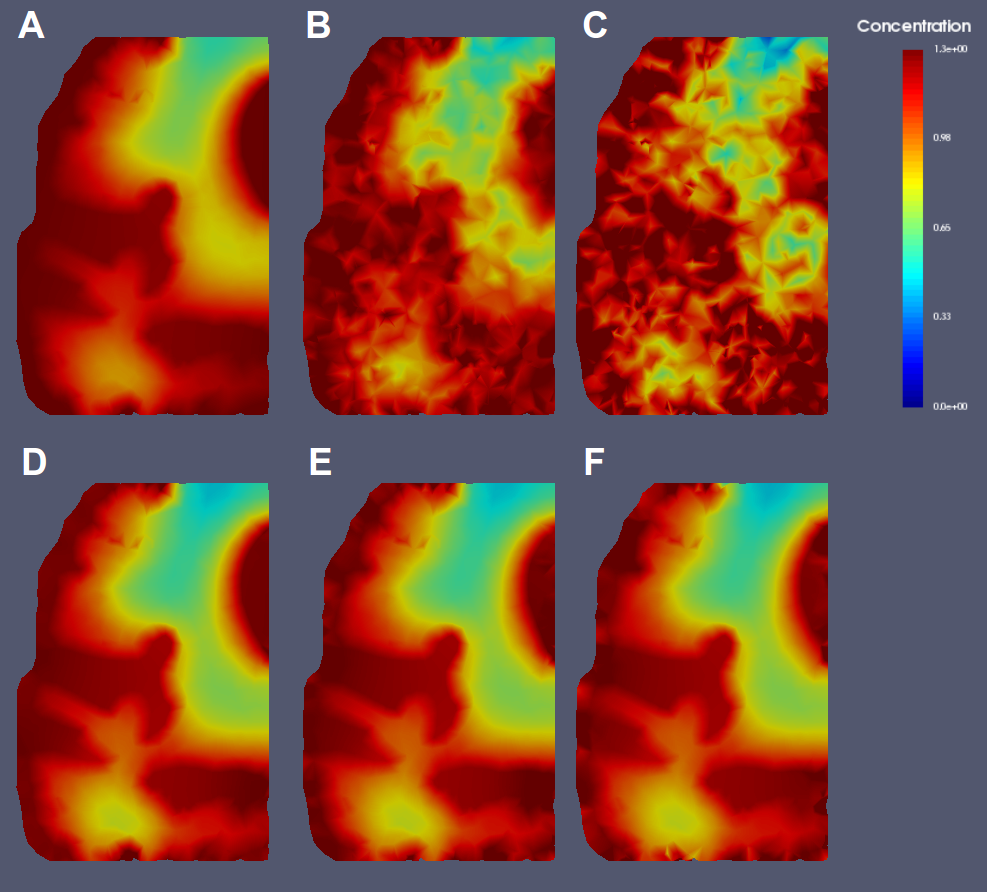
\includegraphics[scale=0.4]{27-12-hours-scale-0-1-3.png}  
%\caption{The upper row shows the manufactured observation, A ) Shows the manufactured observation at time-point 24 with no noise added. B) Shows the manufactured observation at time-point 24 with an noise amplitude of 0.15. C)Shows the manufactures observation at time-point 24 with noise amplitude of 0.3. The lower row shows the results with optimized parameter obtained with $alpha=0.0001$, $\beta=1.0$ and $k=27$. D) Shows the resulting state given the observation in A. E)  Shows the resulting state given the observation in B .F) Shows the resulting state given the observation in C. }
%\end{figure}
%
%
%\begin{figure}
%\centering
%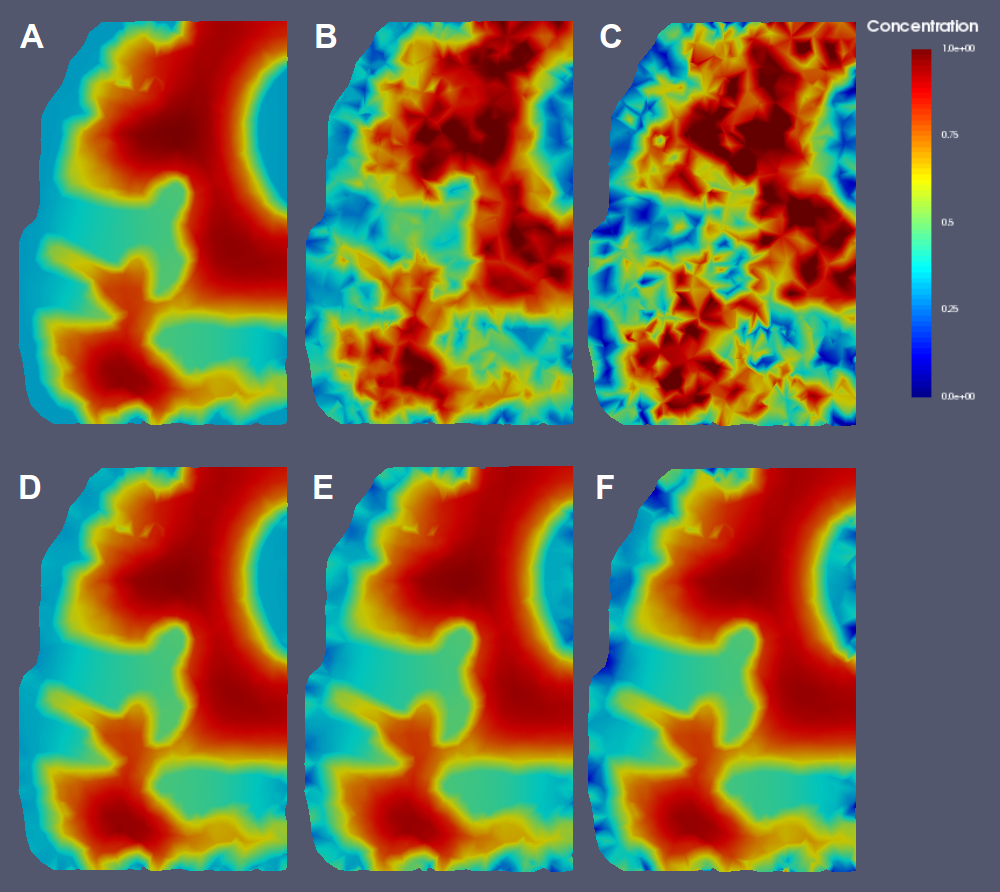
\includegraphics[scale=0.4]{27-24-hours-scale-0-1.png}
%\caption{The upper row shows the manufactured observation, A ) Shows the manufactured observation at time-point 24 with no noise added. B) Shows the manufactured observation at time-point 24 with a noise amplitude of 0.15 {\color{red} explain noise ampliutde}. C)Shows the manufactures observation at time-point 24 with noise amplitude of 0.3. The lower row shows the results with optimized parameter obtained with $alpha=0.0001$, $\beta=1.0$ and $k=27$. D) Shows the resulting state given the observation in A. E)  Shows the resulting state given the observation in B .F) Shows the resulting state given the observation in C.  }
%\end{figure}
% 
% 
% 
%
% 

\subsection{Acknowledgements}
The computational experiments were performed on the Abel Cluster, owned by the University of Oslo and Uninett\textbackslash Sigma2, and operated by the Department for Research Computing at USIT,the University of Oslo IT-department. \url{http://www.hpc.uio.no/} 



%\bibliographystyle{plainnat}
\bibliographystyle{abbrvnat}
\bibliography{references}

 


\clearpage
 
\begin{figure}
\centering
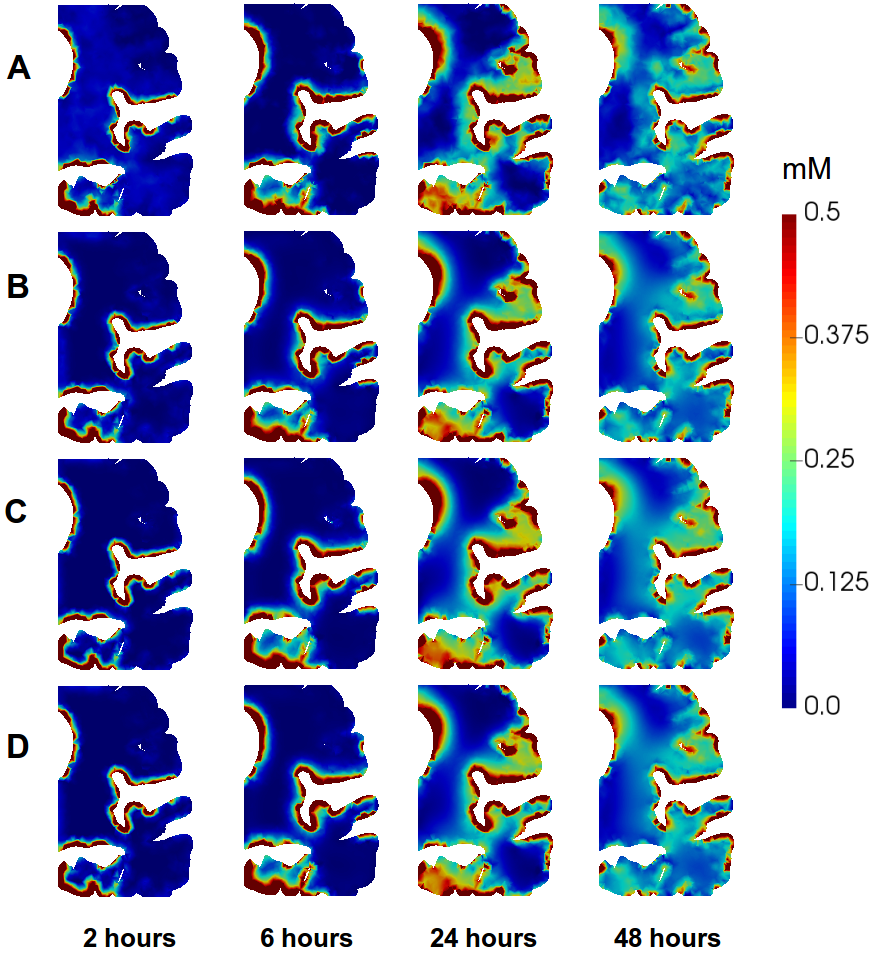
\includegraphics[width=0.95\textwidth]{../different.png} 
\caption{Row A) shows the observation at times 2 hours, 6 hours, 24 hours and 48 hours after the first observation with contrast. Row B) shows the corresponding states with the relaxation parameters $\alpha=0.01$ and $\beta=0.01$ and $k=48$.   Row C) shows the corresponding states with the relaxation parameters $\alpha=1.0\mathrm{e-4}$ and $\beta=1.0$ and $k=48$
 Row D) shows the corresponding states with the relaxation parameters $\alpha=1.0\mathrm{e-6}$ and $\beta=0.1$ and $k=48$. The color-bar was restricted to the range $ \lbrace 0 ,0.5 \rbrace$. }
\label{Fig::realdata}
\end{figure}

\begin{figure}
\centering
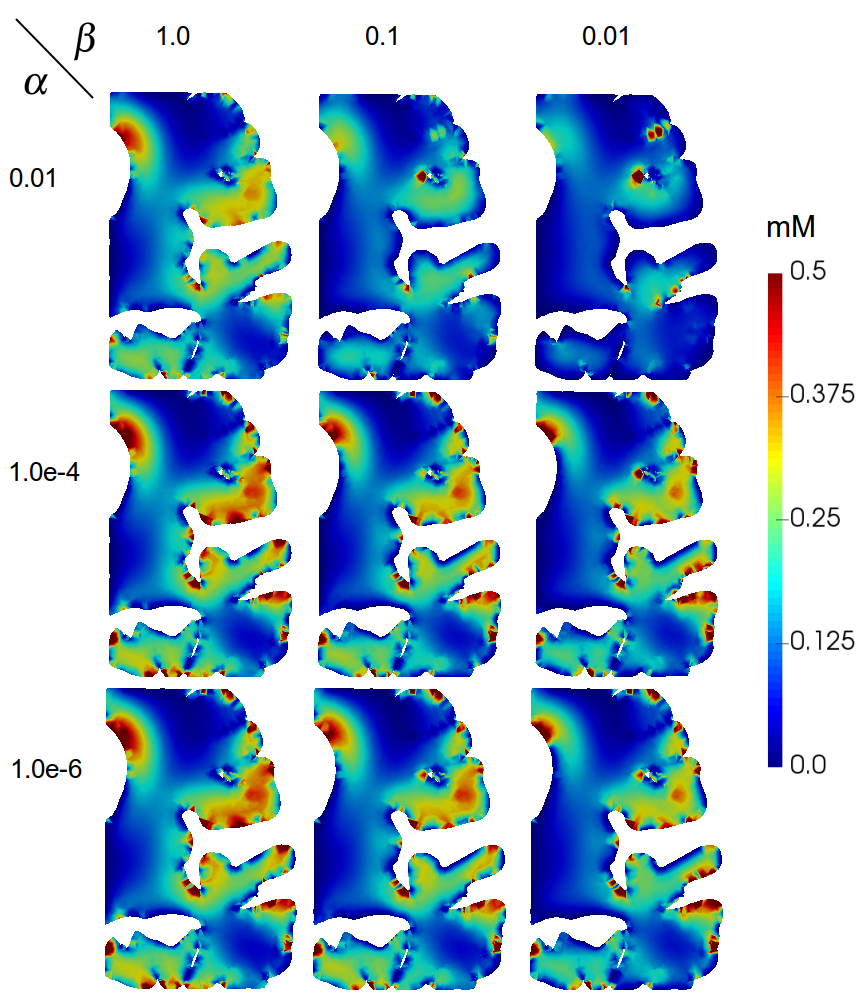
\includegraphics[width=0.95\textwidth]{../Statecomparison36h-pinta.png} 
\caption{ Displays the states for different regularization parameters after 36 hours for $k=48$.}
\label{statecomparison}
\end{figure}

 
 \begin{figure}
\centering
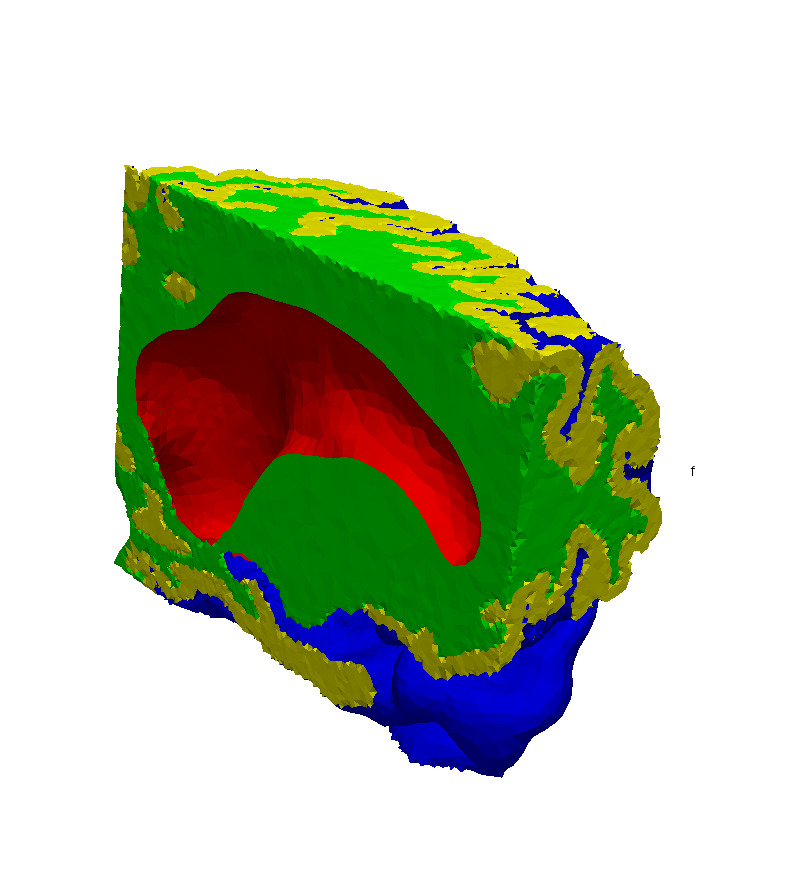
\includegraphics[scale=0.3]{../facetfucntion.png} 
\caption{The images shows the marked boundary values on the mesh. }
\label{markedboundaryvalues}
\end{figure}

\begin{figure}
\centering
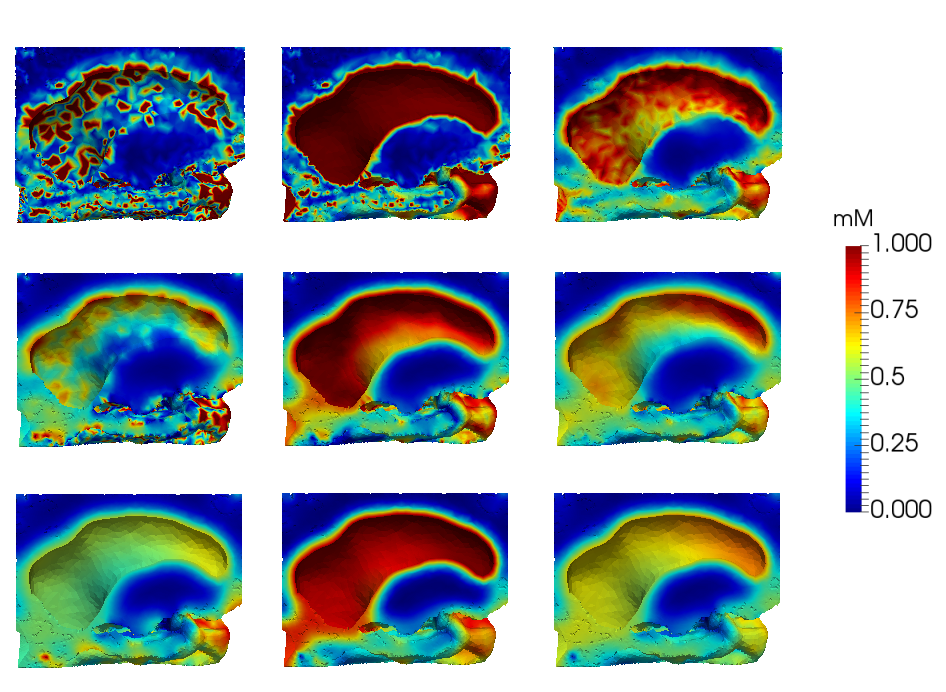
\includegraphics[scale=0.35]{../Vent-2.png} 
\caption{ The images shows the ventricular wall at the same time points. The upper row shows the observations with following preprocessing left to right: Raw observations, projection of CSF value onto the boundary, Gaussian smoothing. The middle row shows the corresponding states with the regularization parameters $\alpha , \beta \gamma = (10\sp{-6},1.0 ,1.0)$. The bottom row shows the corresponding states with the regularization parameters $\alpha , \beta \gamma = (10\sp{-6},100.0 ,100.)$. }
\label{VENT}
\end{figure}

\begin{figure}
\centering
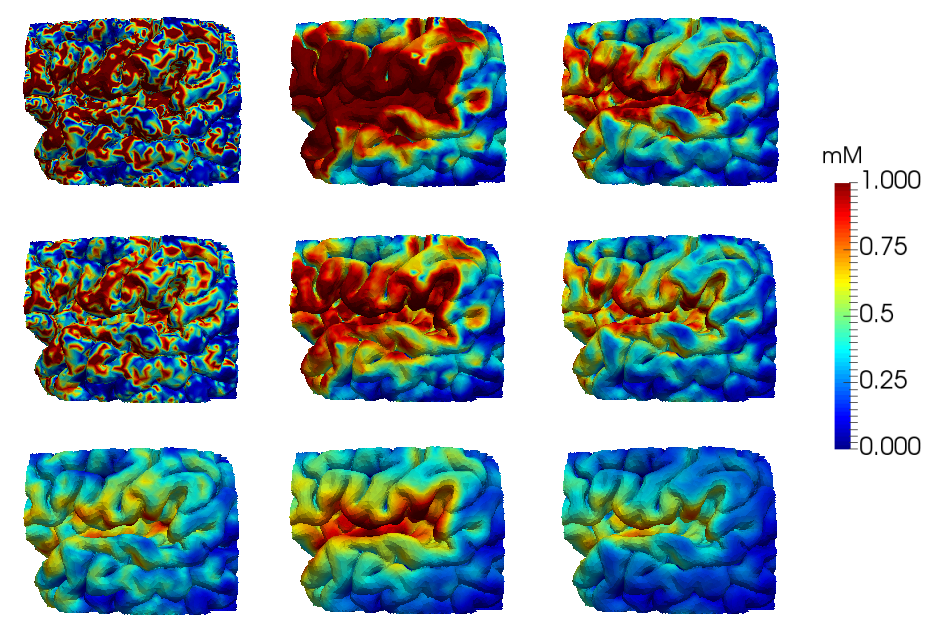
\includegraphics[scale=0.35]{../SAS-2.png} 
\caption{ The images shows the SAS boundary at the same time points. The upper row shows the observations with following preprocessing left to right: Raw observations, projection of CSF value onto the boundary, Gaussian smoothing. The middle row shows the corresponding states with the regularization parameters $\alpha , \beta \gamma = (10\sp{-6},1.0 ,1.0)$. The bottom row shows the corresponding states with the regularization parameters $\alpha , \beta \gamma = (10\sp{-6},100.0 ,100.)$. }
\label{SAS}
\end{figure}

\begin{figure}
\centering
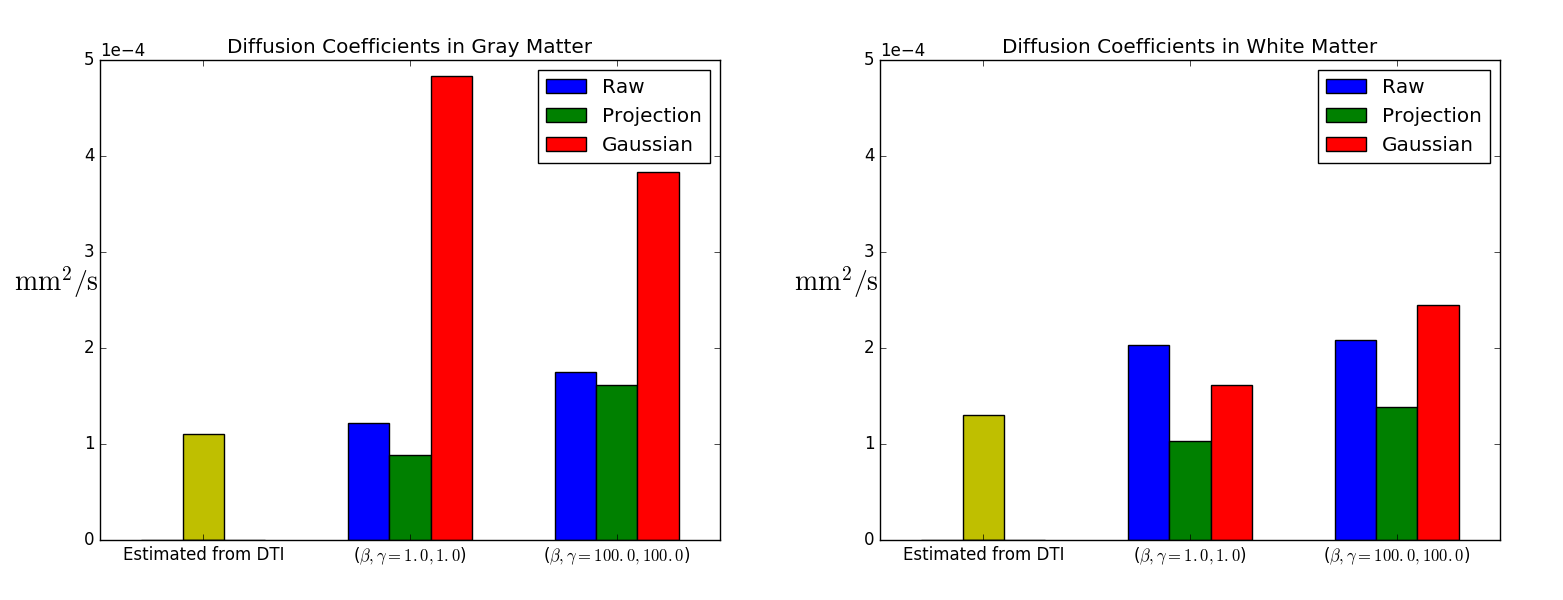
\includegraphics[scale=0.3]{../diffcoeff.png} 
\caption{The images shows the computed diffusion coefficients in gray and white matter given different preprocessing steps.  }
\label{diffcoeff}
\end{figure}


\clearpage
\section{Supplementary}

\subsection{Testing with a manufactured solution to assess accuracy.}
\label{sup:manu}

Below we will discuss the parameter identification and its sensitivity with respect to the regularization parameters, noise, number of observations and time-resolution of the forward model. 
The manufactured observations were obtained by forward computation of \eqref{Eq::PDE} with the Dirichlet boundary condition defined as 
\begin{equation}
g(t) = 0.3 +0.167t - 0.007t\sp{2} \qquad \text{ for } 0 \leq t \leq 24.
\label{EQ::DIRI}
\end{equation}
The initial condition was set to 0 everywhere, the timestep was $dt = 0.2$, and the diffusion coefficients were selected to be 
\begin{equation}
D_{\Omega_1} = 1000.0, \quad D_{\Omega_2} = 4.0, \quad D_{\Omega_3} = 8.0 
\end{equation}  

\begin{figure}
\centering
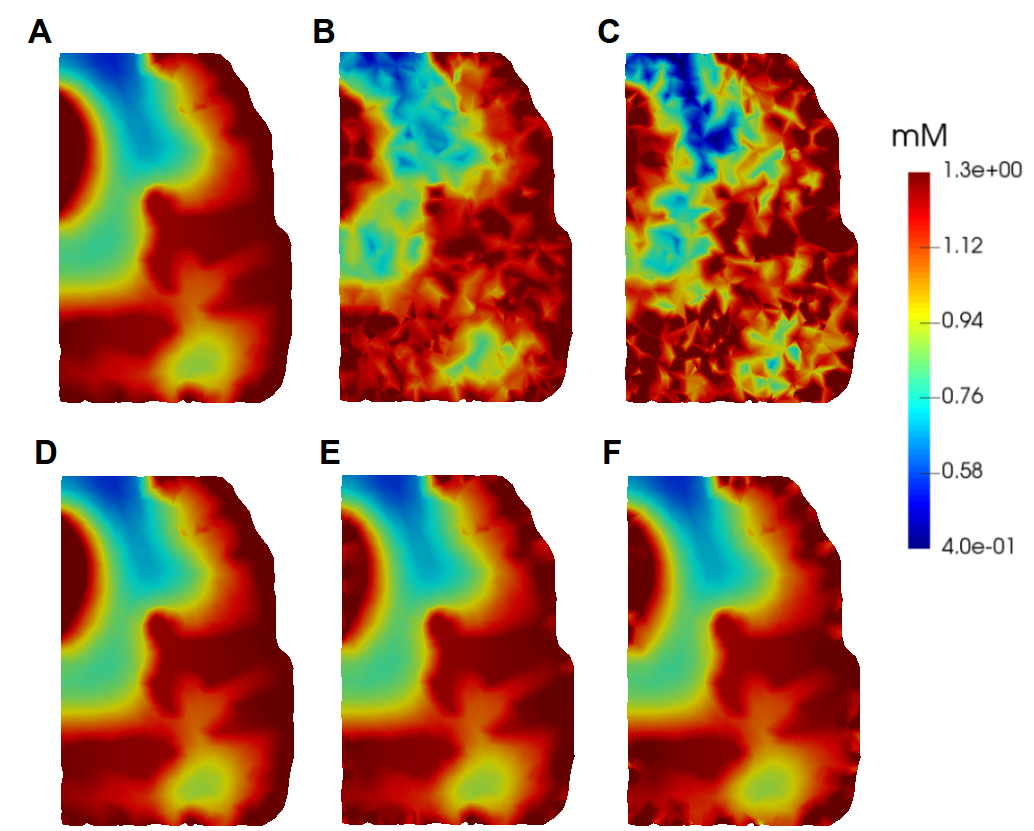
\includegraphics[scale=0.4]{noise-12.png}  
\caption{The upper row shows the manufactured observation, A) Shows the manufactured observation at time-point 24 with no noise added. B) Shows the manufactured observation after 12 hours with noise amplitude of 0.15. C) Shows the manufactures observation after 12 hours with noise amplitude of 0.3. The lower row shows the results with optimized parameter obtained with $\alpha=0.0001$, $\beta=1.0$ and $k=20$. D) Shows the resulting state given the observation in A. E)  Shows the resulting state given the observation in B .F) Shows the resulting state given the observation in C. }
\label{12hourswithnoise}
\end{figure}





\subsection{Contrast concentration - Image Signal Relation}
Below, we briefly describe the relationship between the imaging signal 
seen in Figures~\ref{fig1} and \ref{fig2} and the underlying contrast 
concentration. We remark that we use a notation common in medical literature and here two letter symbols are common. Hence, below we will use two letter symbols such as $TE$ and $TR$ to keep the notation consistent with the presentation in \cite{GOWLAND, MPRAGE}.   
The contrast concentration $c$ causes the longitudinal(spin-lattice) relaxation time $T_{1}$ to shorten with the following relation
\begin{equation}
\frac{1}{T_{1}\sp{c}} = \frac{1}{T_{1}\sp{0}} + r_{1}c .
\label{EQ::contrast}
\end{equation}
The superscripts indicate relaxation time with contrast $T_{1}\sp{c}$ and without contrast $T_{1}\sp{0}$, and $r_1$ is the relaxivity constant for the MRI-contrast in a medium. 
The contrast observations were collected using a MRI sequence known as  Magnetization Prepared Rapid Acquisition Gradient Echo (MPRAGE) with an inversion prepared magnetization. The relation between signal and the relaxation time is non-linear, and is expressed with the following equations. The signal value $S$ for this sequence is given by
\begin{equation}
S = M_{n} \sin \theta e\sp{ - TE/T_2\sp{*} },
\label{EQ::SI_T2}
\end{equation}
with $TE$ and $\theta$ respectively denoting the echo time and the flip angle, and $M_{n}$ the magnetization for the n-echo described below. 
Also $T_2\sp{*}$ is transverse magnetization caused by a combination of spin-spin relaxation and magnetic field inhomogeneity. It is defined as 
\begin{equation}
\frac{1}{T_2\sp{*}} = \frac{1}{T_2} + \gamma \Delta B_{in} ,
\end{equation}
with $T_2$ transverse (spin-spin) relaxation time, $\gamma$ is the gyromagnetic ratio and $\Delta B_{in}$ is the magnetic field inhomogeneity across a voxel. The expression can be simplified by neglecting the $T_2$ term in the signal, since $TE <<T_2\sp{*}$ for this MRI sequence. Thus \eqref{EQ::SI_T2} becomes 
\begin{equation}
S = M_{n} \sin \theta.
\label{EQ::SI}
\end{equation}
In article \cite{GOWLAND}, the term $M_n$ is defined as the magnetization for the n-echo 
\begin{equation}
M_{n} = M_{0}  \left[ (1-\beta)\frac{(1-(\alpha \beta)\sp{n-1} }{1-\alpha\beta} + (\alpha \beta)\sp{n-1}(1-\gamma) + \gamma ( \alpha \beta)\sp{n-1} \frac{M_{e}}{M_{0}}  \right]   
\end{equation}
with 
\begin{equation}
\frac{M_{e}}{M_{0}} = - \left[ \frac{ 1 -\delta + \alpha \delta (1-\beta ) \frac{1-\alpha\beta\sp{m}}{1-\alpha \beta} + \alpha\delta(\alpha\beta)\sp{m-1} - \alpha\sp{m}\rho}{1 +\rho \alpha\sp{m} } \right].
\end{equation}
Using the following definitions
\begin{equation}
\begin{aligned}
\alpha &= \cos ( \theta ) \\
\beta  &= e\sp{- \sp{T_b}/_{T_1\sp{c}} } \\
\delta &= e\sp{- \sp{T_a}/_{T_1\sp{c}} } \\
\gamma &= e\sp{- \sp{T_w}/_{T_1\sp{c}} } \\
\rho   &= e\sp{- \sp{TR}/_{T_1\sp{c}}}  \\
T_w    &= TR - T_a -T_b(m-1)       .\\
\end{aligned}
\end{equation}
Here $T_b$ is known as the echo spacing time, $T_a$ is the inversion time, $T_w$ the time delay, $TR$ as the repetition time, $m$ is the number of echo spacings and $M_0$ is a calibration constant for the magnetization. The center echo denoted as $n=m/2$ will be the signal that we will consider when estimating MRI-contrast. Given \eqref{EQ::SI} we have that the relative signal increase can be written as 
\begin{equation}
\frac{S\sp{c}}{S\sp{0}} = \frac{ M_{n}\sp{c} \sin (\theta)}{ M_{n}\sp{0} \sin (\theta) }.
\end{equation}
We define that  
\begin{equation}
f(T_1) = M_{n}/M_{0} ,
\label{scaledmagnetization}
\end{equation}
which can be seen in Figure~\ref{figuredti}. 
This gives the following relation 
\begin{equation}
\frac{f(T_{1}\sp{c} ) }{f(T_{1}\sp{0})}  = \frac{S\sp{c}}{S\sp{0}} 
\end{equation}
The signal difference between observation times were adjusted in \cite{ringstad2018brain}. Thus we can express the change in $T_1$ due to contrast as 
\begin{equation}
f ( T_{1}\sp{c} ) = \frac{S\sp{c}}{S\sp{0}} f(T_{1}\sp{0}) 
\end{equation}
and then estimate the concentration using \eqref{EQ::contrast}. The $T_{1}\sp{0}$ values were obtained by T1-mapping of the brain using a MRI sequence known as MOLLI5(3)3 \cite{TAYLOR201667}. This takes into account patient specific characteristic, such as tissue damage. Tissue damage can be observed in the MRI due to a lower signal in the white matter compared to healthy white matter tissue, thus damaged tissue have different $T_1$ relaxation time. 
The contrast concentration was estimated in a preprocessing step, using the parameters obtained from the T1-map, MPRAGE MRI protocol \cite{ringstad2018brain} and the value for $r_1$ found in \cite{pmid16230904}. In the computation, the function \eqref{scaledmagnetization} was computed for $ T_1\in \lbrace 200, 4000 \rbrace$ creating a lookup table. The lookup table was utilized with the baseline signal increase to estimate $T_1\sp{c}$, and then the concentration was computed using \eqref{EQ::contrast}.  

\begin{figure}
\centering
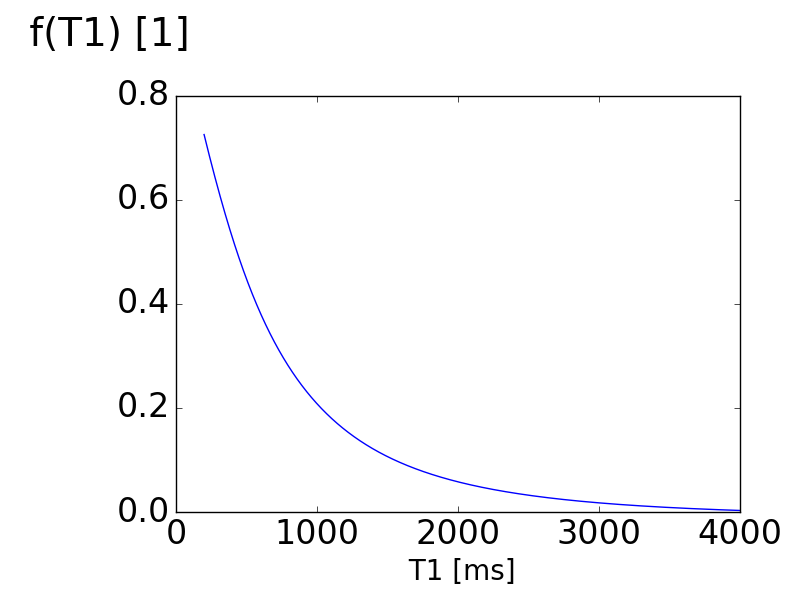
\includegraphics[width=0.70\textwidth]{../T1function.png} 
\caption{Shows the  function defined in \eqref{scaledmagnetization} where the white region indicates $T_1$ values for white matter, the grey region indicates $T_1$ values for grey matter, the blue region indicates $T_1$ values for CSF.  }
\label{figureF} 
\end{figure}


\subsection{Diffusion tensor imaging}
In addition to the T1 and T2 weighted sequences described above we have also obtained diffusion tensor imaging to assess the apparent diffusion 
coefficients on short time-scales. Images are shown in Figure~\ref{figuredti} where the largest diffusion coefficient (shown in 
red in the middle figure) is shown to be around $1.0\mathrm{e}{-3}  \mathrm{mm^2/s}$. We remark that we have not included possible anisotropy, shown in 
the right-most image in Figure~\ref{figuredti} and that these images show the apparent diffusion coefficient for free water molecules (18 Da).      
The diffusivity of the Gadovist (600 Da) \cite{MGadobutrol} was estimated to be similar to the diffusion coefficient of Gd-DPTA (550 Da) \cite{MGgDPTA}. This is due to the fact that both molecules have similar mass, and based on Stoke-Einstein equation should also have similar diffusion coefficients. The free diffusion coefficient for Gd-DPTA was estimated in \citet{GdDPTA-DIFFUSION} to be $3.8\mathrm{e}{-4}\mathrm{mm\sp{2}/s}$.
The fractional anisotropy is defined as 
\begin{equation}
FA\sp{2} =  \frac{3}{2} \frac{ (\lambda_1 - MD )\sp{2} +(\lambda_2 - MD )\sp{2} +(\lambda_3 - MD )\sp{2}}{\lambda\sp{2}_1 + \lambda\sp{2}_2  +\lambda\sp{2}_3 },
\end{equation}
with the mean diffusivity $MD$ defined as 
\begin{equation}
MD = \frac{\lambda_1 +\lambda_2 +\lambda_3 }{3}.
\end{equation}
In these equations $\lambda_i$ denotes the eigenvalues of the diffusion tensor.
\begin{figure}
\centering
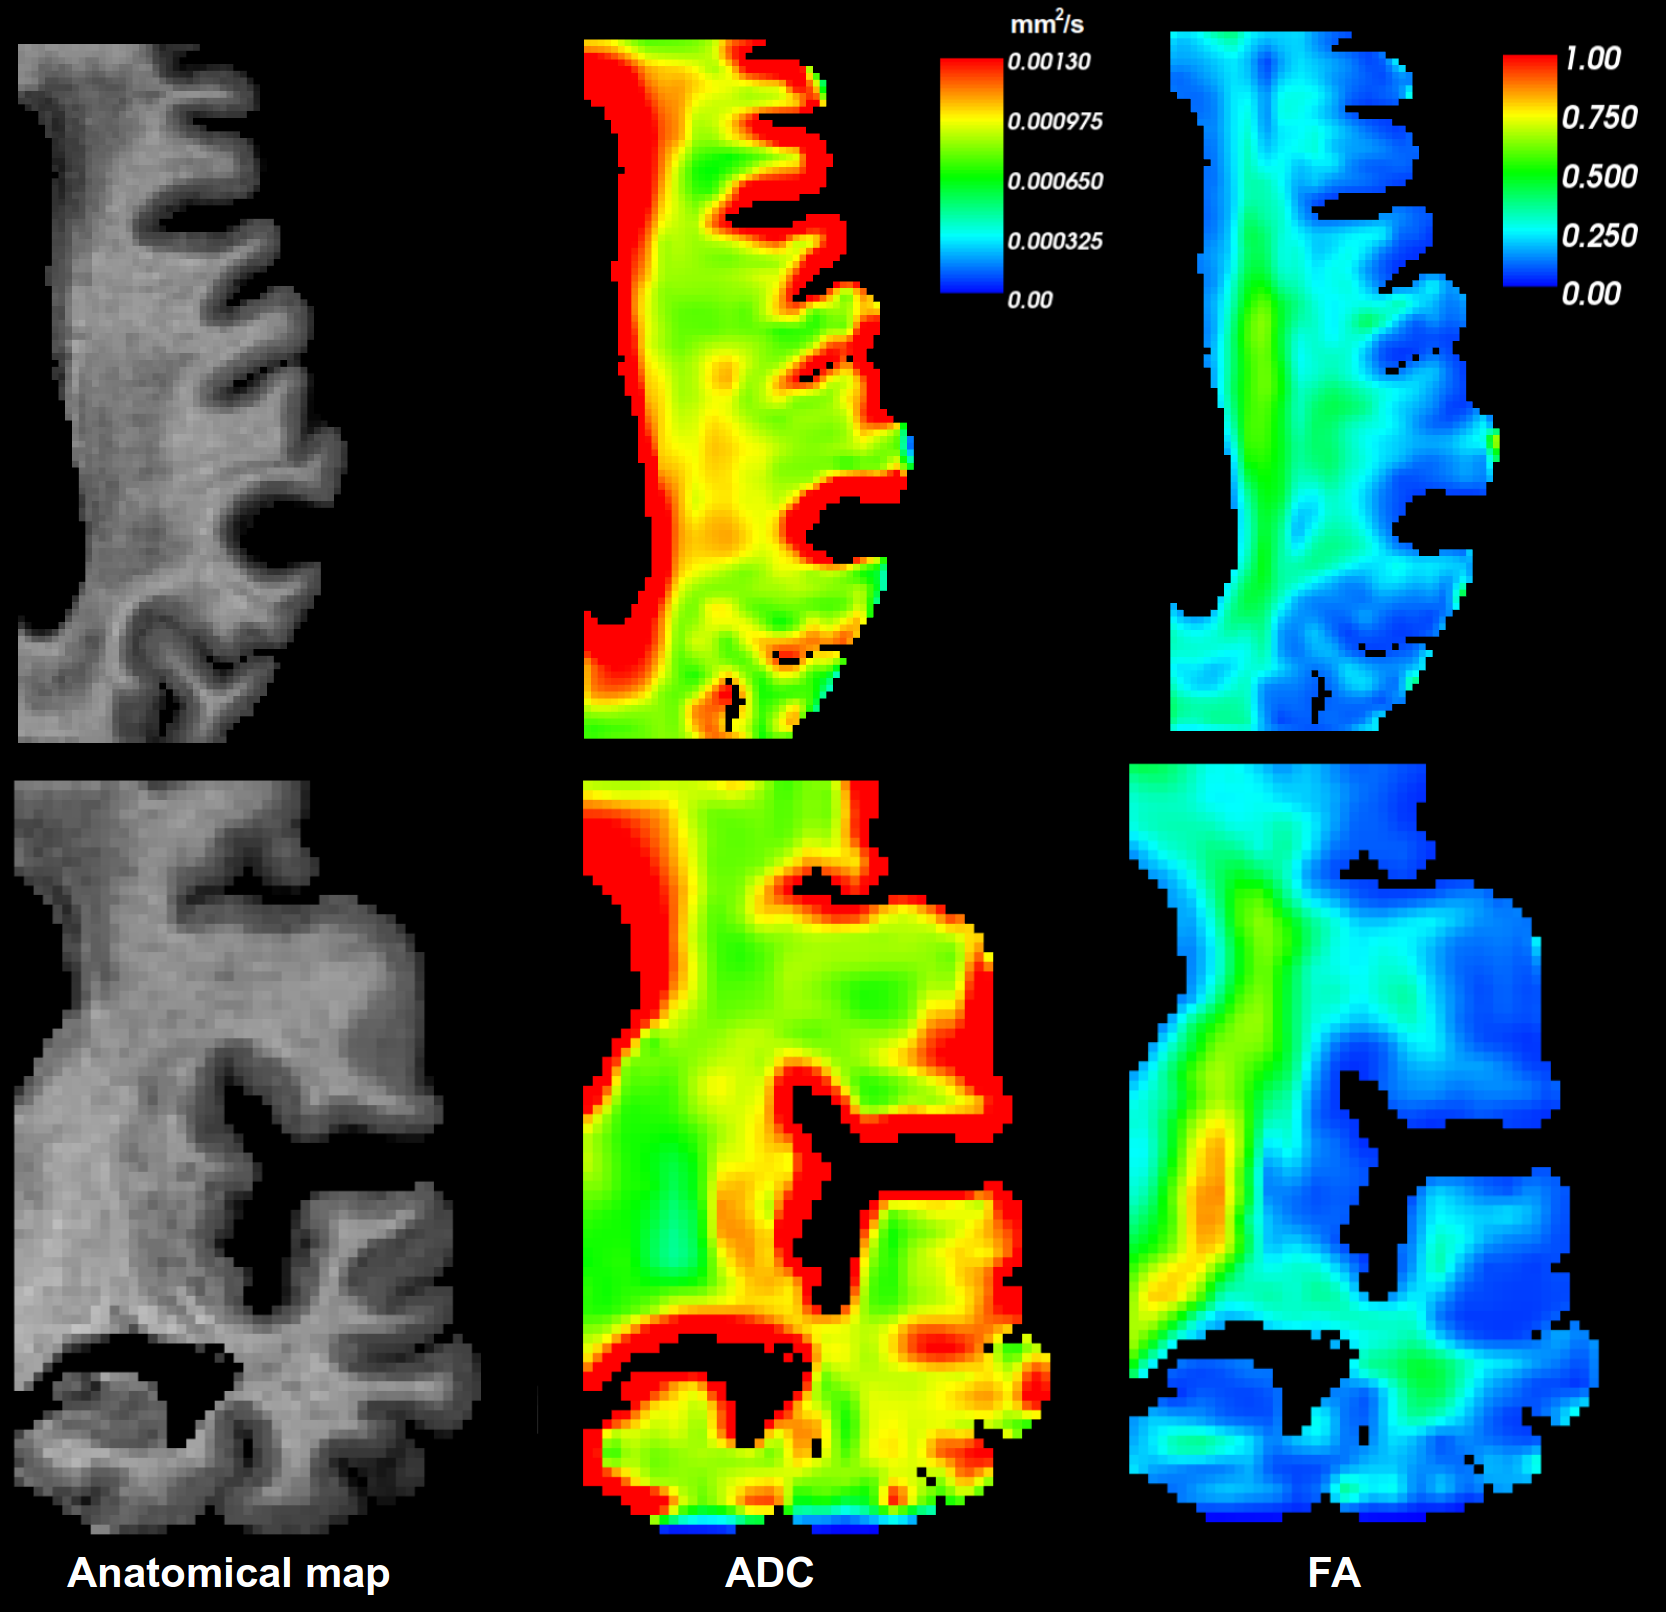
\includegraphics[width=0.75\textwidth]{../DTI-zoom.png} 
\caption{The left panel shows the anatomical map. The middle panel shows the apparent diffusion coefficients (ADC) obtained from DTI. The right panel shows the computed fractional anisotropy (FA) from the DTI.}
\label{figuredti} 
\end{figure}



\section{





\end{document}


